\thispagestyle{lichsutoanhocnone}
\pagestyle{lichsutoanhoc}
\graphicspath{{../lichsutoanhoc/pic2/}}
\everymath{\color{lichsutoanhoc}}
\blfootnote{$^1$\color{lichsutoanhoc}THPT chuyên Hà Nội -- Amsterdam.}
\begingroup
\AddToShipoutPicture*{\put(0,616){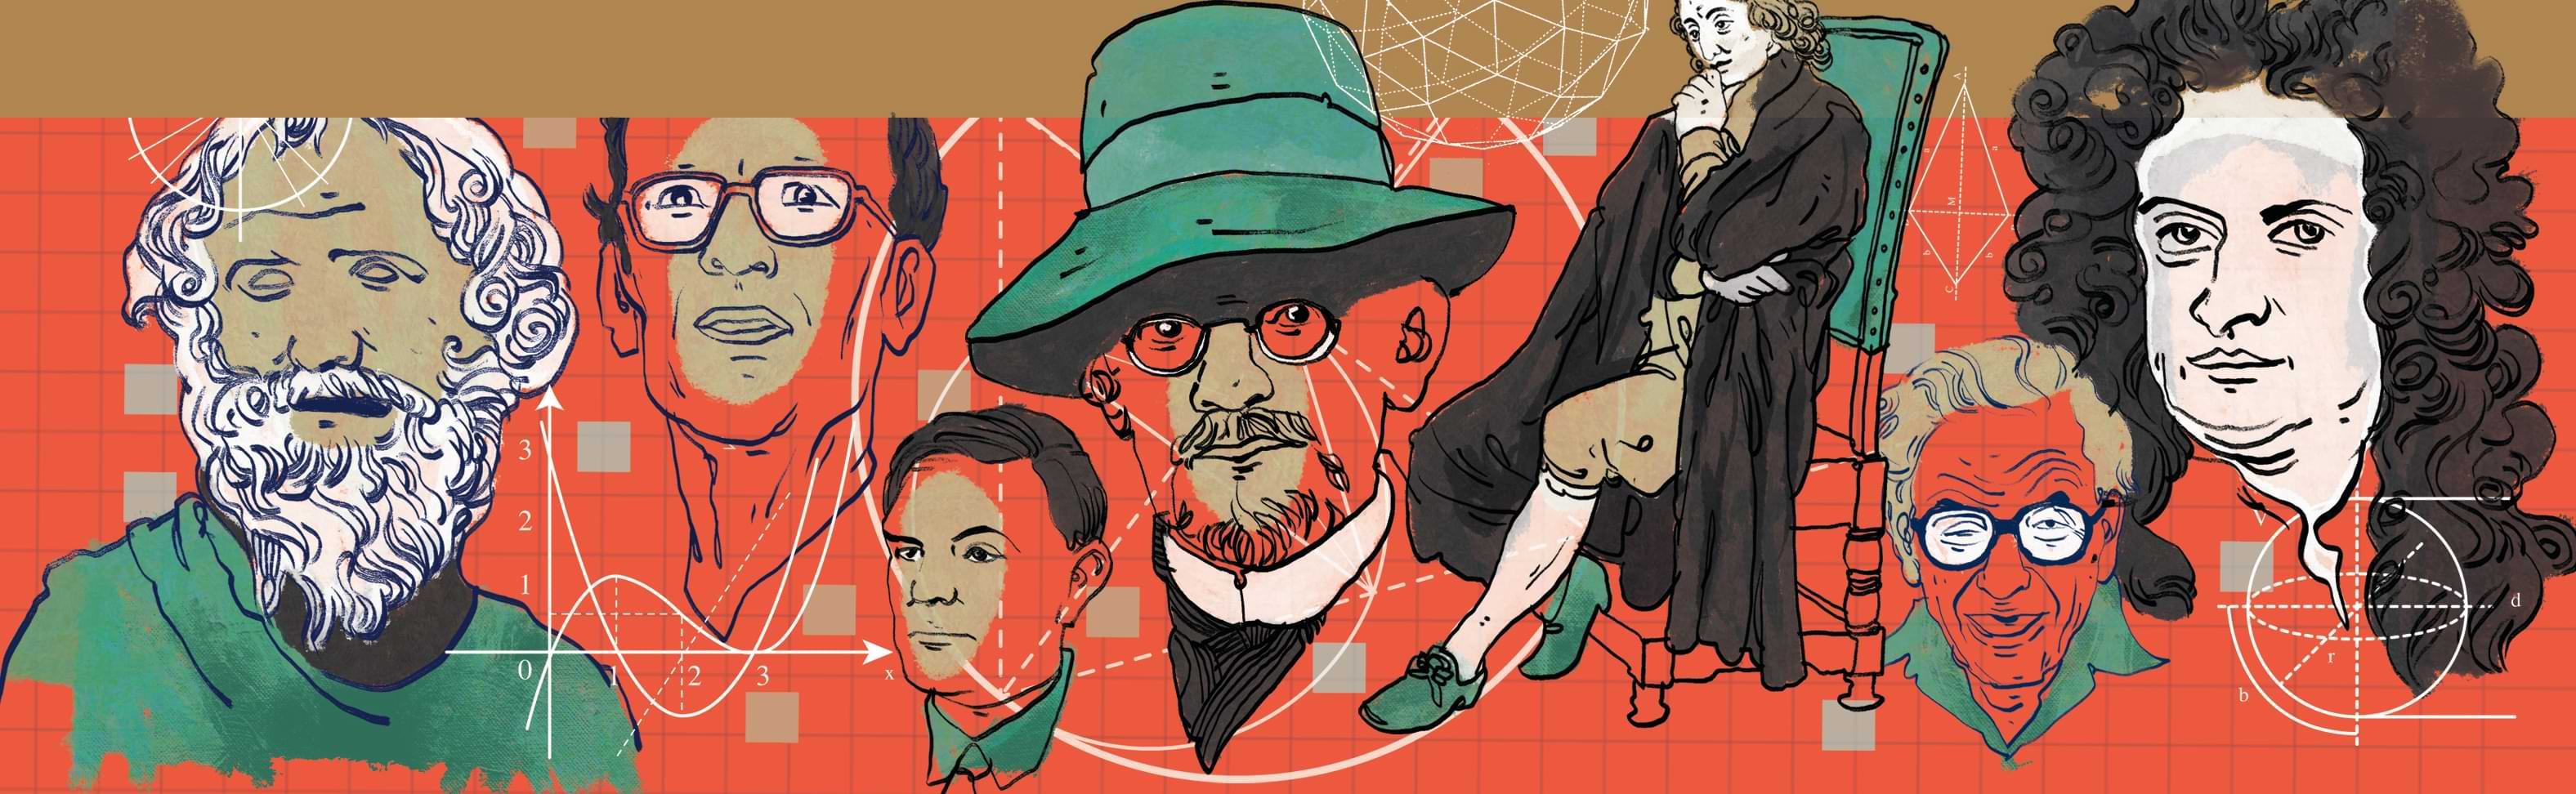
\includegraphics[width=19.3cm]{../bannerlichsu}}}
\AddToShipoutPicture*{\put(82,555){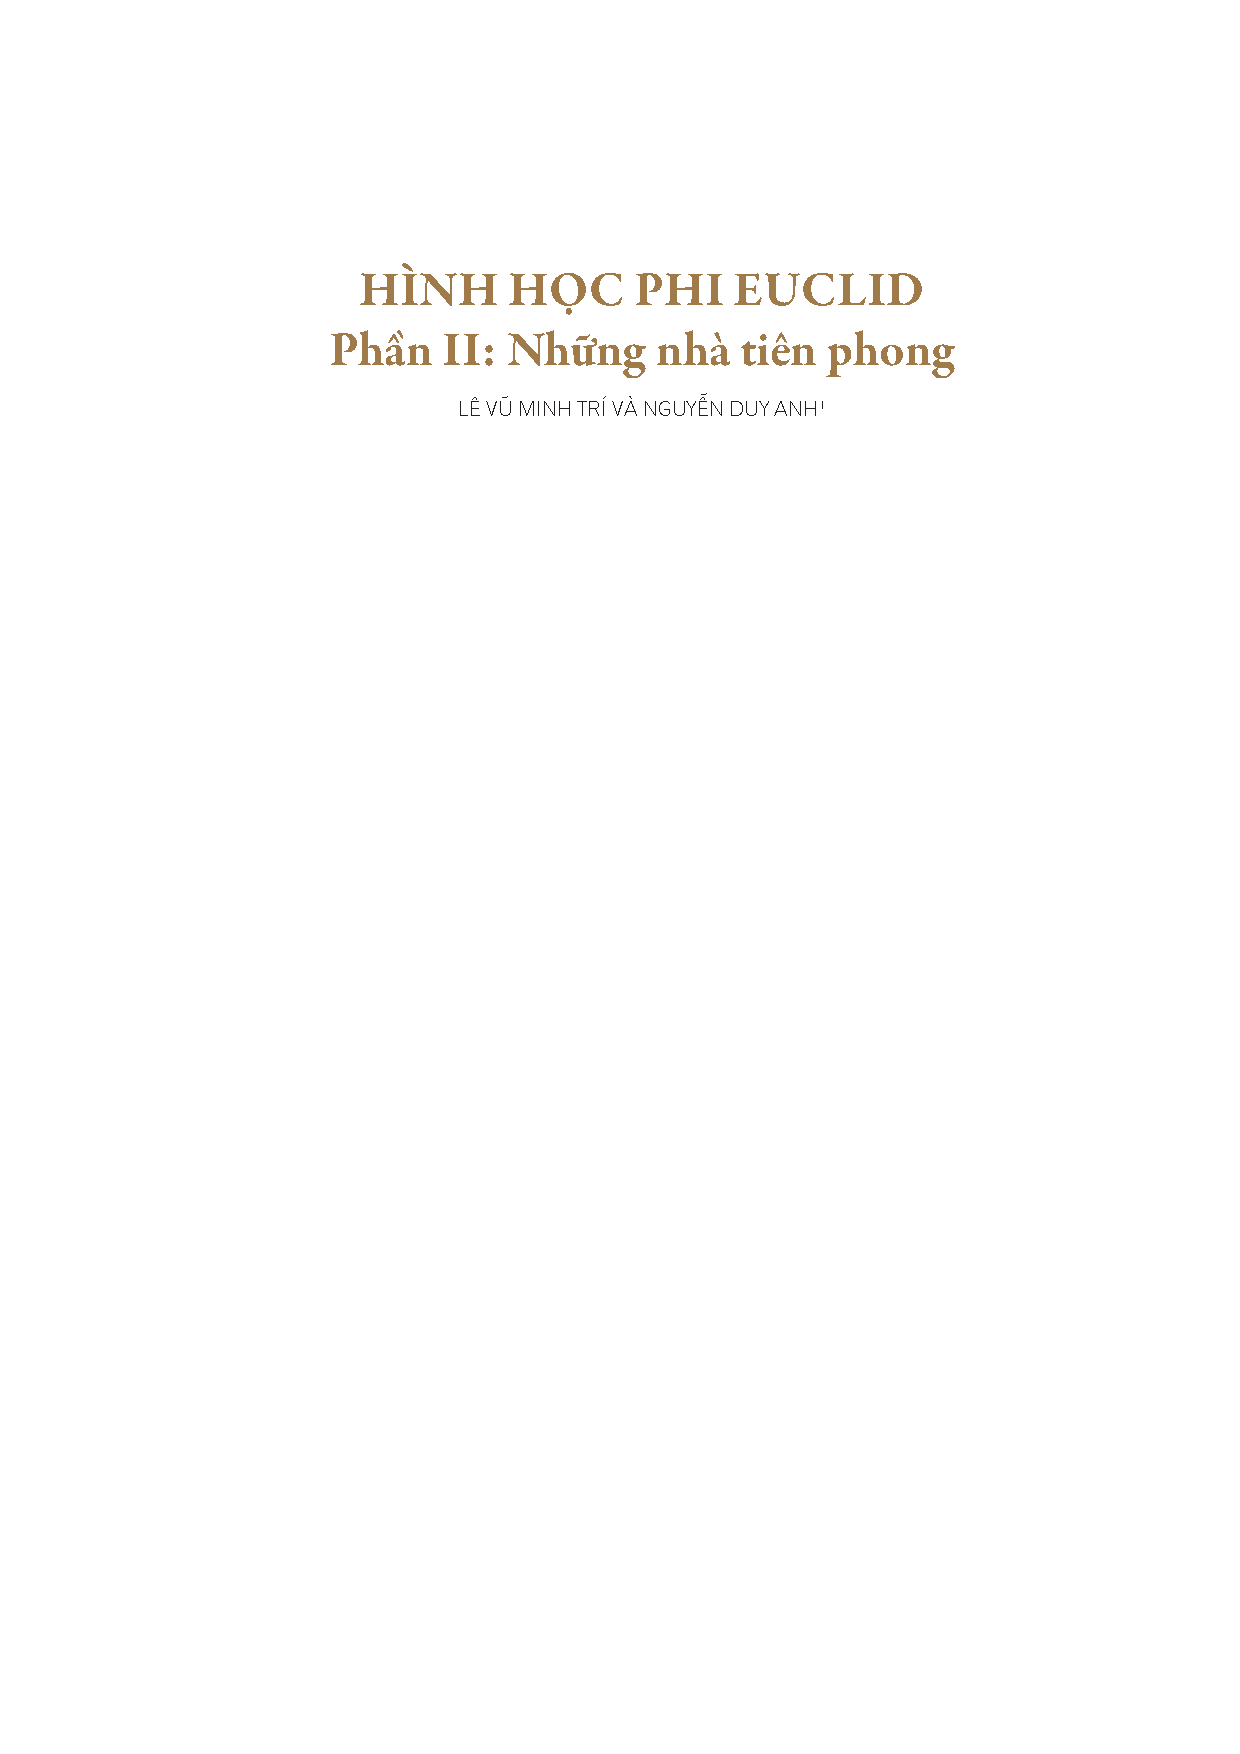
\includegraphics[scale=1]{../tieude3.pdf}}}
\centering
\endgroup

\textbf{Hiệp: sửa tiêu đề thành}

{Hình học phi Euclid\\
Phần IV: Hình học trên đĩa Poincaré}
 
	\vskip 0.1cm
	$\pmb{7.}$ \textbf{\color{lichsutoanhoc}Mô hình đĩa Poincar\'e}
	\vskip 0.1cm
 Poincar\'e ($1854 - 1912$), một nhà toán học đa năng, tác giả một trong bảy Bài toán thiên nhiên kỷ, có những điểm của hình hyperbolic được diễn giải như ở mô hình Beltrami--Klein -- ấy là các điểm nằm bên trong một đường tròn $\gamma $ cố định nào đó. Ta gọi đây là mô hình Poincar\'e cho ngắn gọn, dù ông còn một mô hình khác của hình hyperbolic là mô hình nửa mặt phẳng. 
 	\vskip 0.1cm
	Các ``đường thẳng'' sẽ được diễn giải khác. Cụ thể, với hai điểm $A$, $B$ cùng nằm trên một đường kính nào đó của $\gamma$, ``đường thẳng'' đi qua $A$ và $B$ ở đây được định nghĩa là đường kính của $\gamma$ đi qua $A$ và $B$ và bỏ đi hai đầu mút. Trong các trường hợp còn lại thì cung mở trong $\gamma$ của đường tròn trực giao với $\gamma$ và đi qua $A$ và $B$ sẽ là ``đường thẳng'' đang nói. $(O_1)$ và $(O_2)$ được gọi là trực giao nếu như chúng có giao điểm $Y$ và $ \angle O_1YO_2 = 90$. Ta gọi những đường thẳng định nghĩa như trên là đường thẳng Poincaré, viết tắt là đường $P$. 
		\vskip 0.1cm
	Quan hệ ``nằm trên'' có nghĩa như trong hình Euclid. Một lợi thế lớn của mô hình Poincar\'e là tính chất ``bảo giác'' hay bảo toàn góc của nó, bởi ta chỉ cần đơn giản quy ước góc giữa hai đường thẳng trong hình học hyperbolic là góc giữa hai đường  $P$ theo nghĩa trong hình học Euclid. Về sau, chúng tôi sẽ chỉ ra góc giữa hai đường không phải đường thẳng là gì, và tính chất bảo giác và từ đó là bảo toàn tỷ số kép của phép nghịch đảo. Đây chính là điểm then chốt làm nên mô hình đĩa Poincar\'e.
		\vskip 0.1cm
	Sau đây là một vài hình vẽ minh họa cho một số điểm khác biệt so với hình Euclid của hình hyperbolic.
\vskip 0.1cm
\begin{figure}[ht]
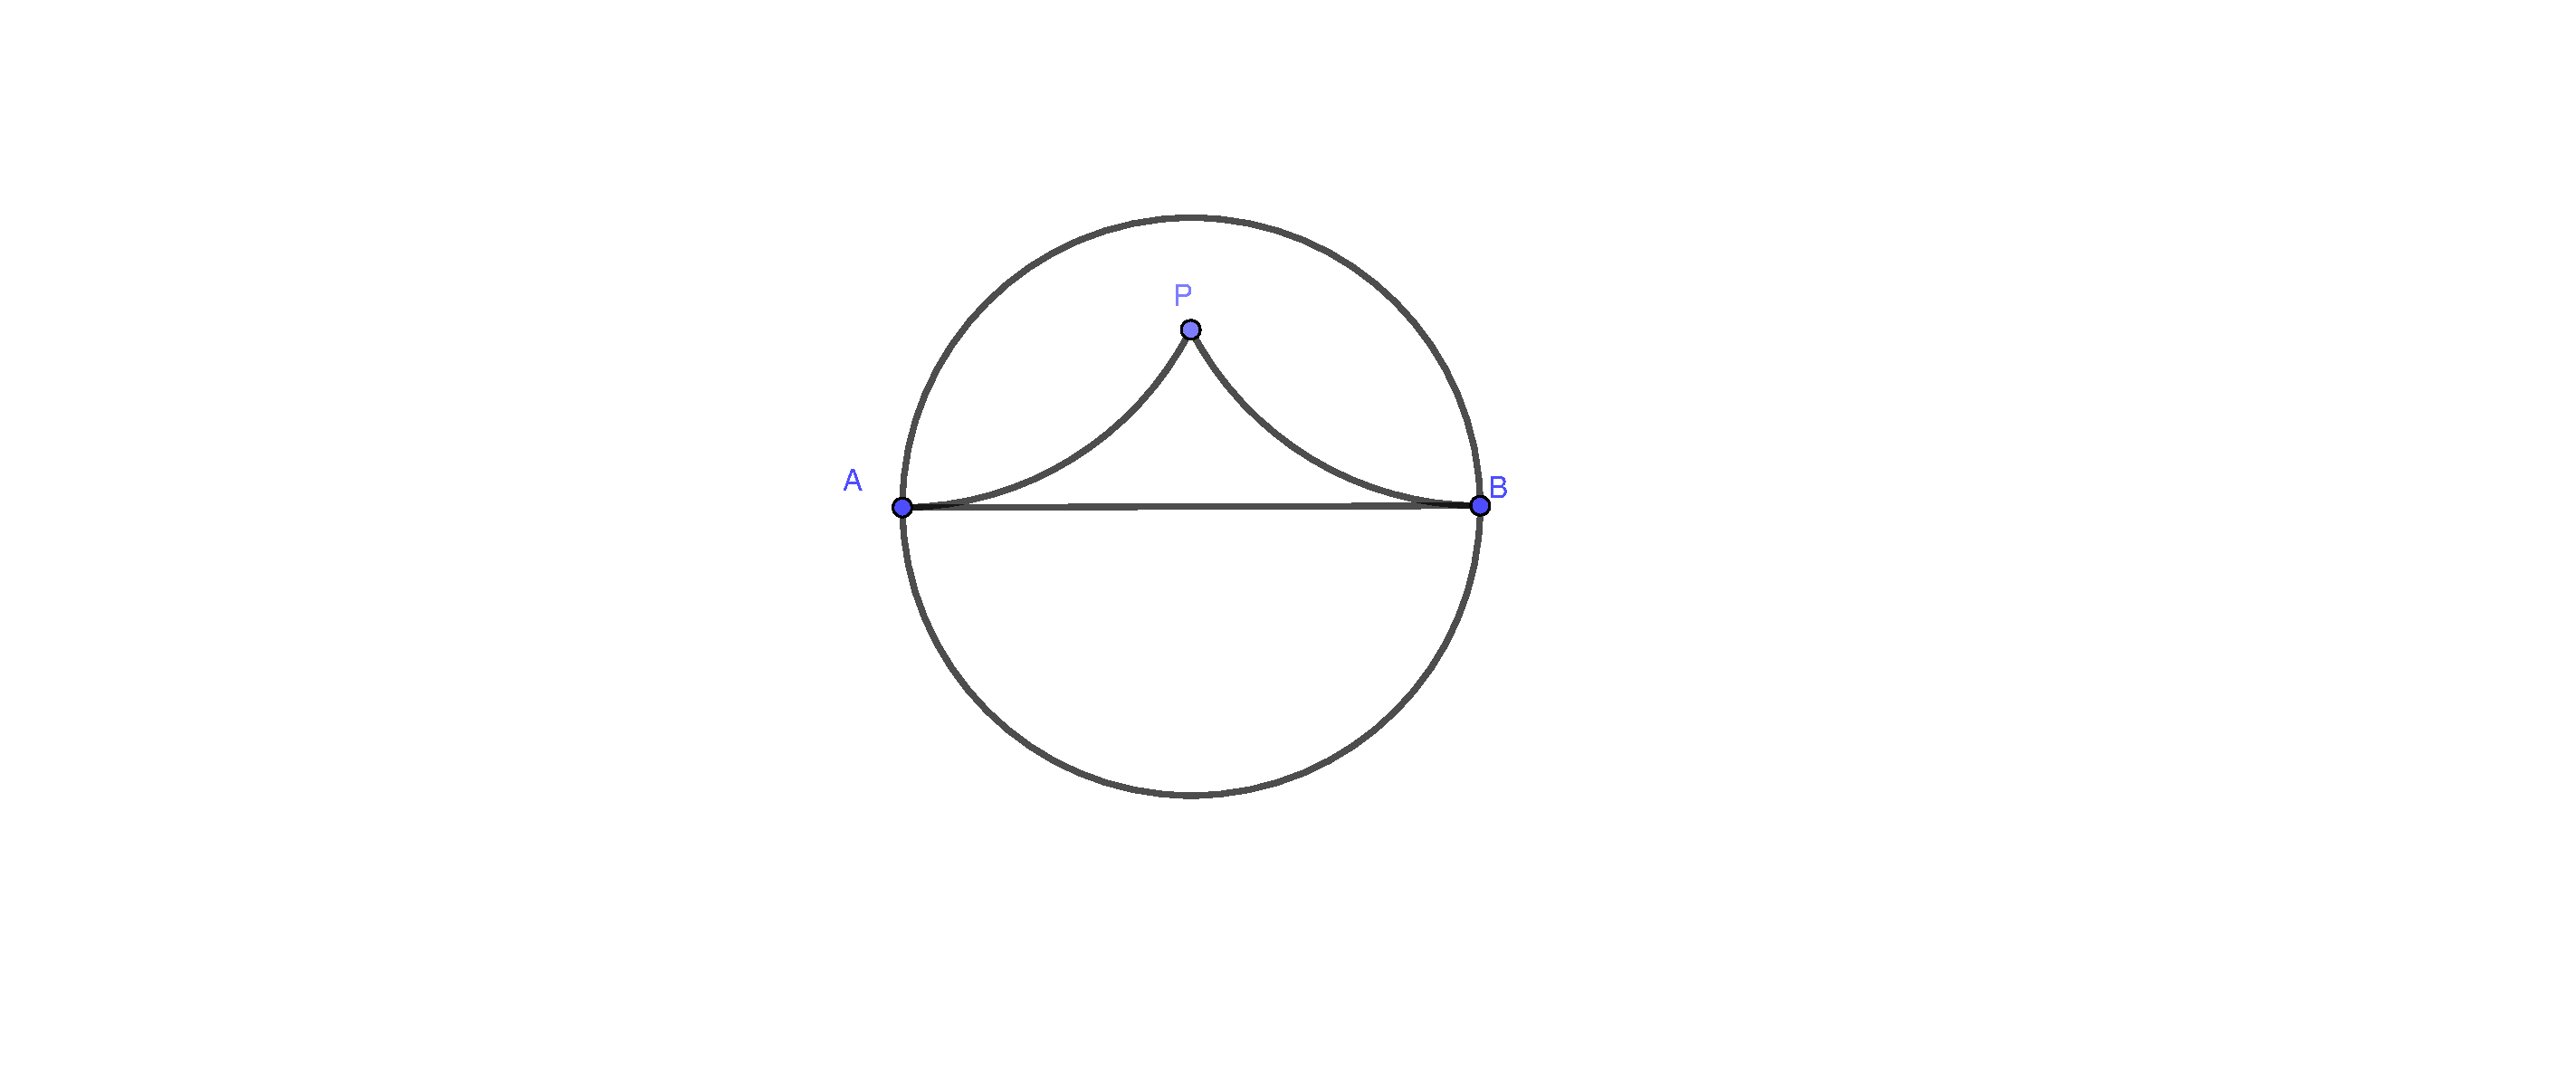
\includegraphics[width=\textwidth]{Duong_song_song_gioi_han_Poincare.pdf}
\end{figure}

\begin{figure}[ht]
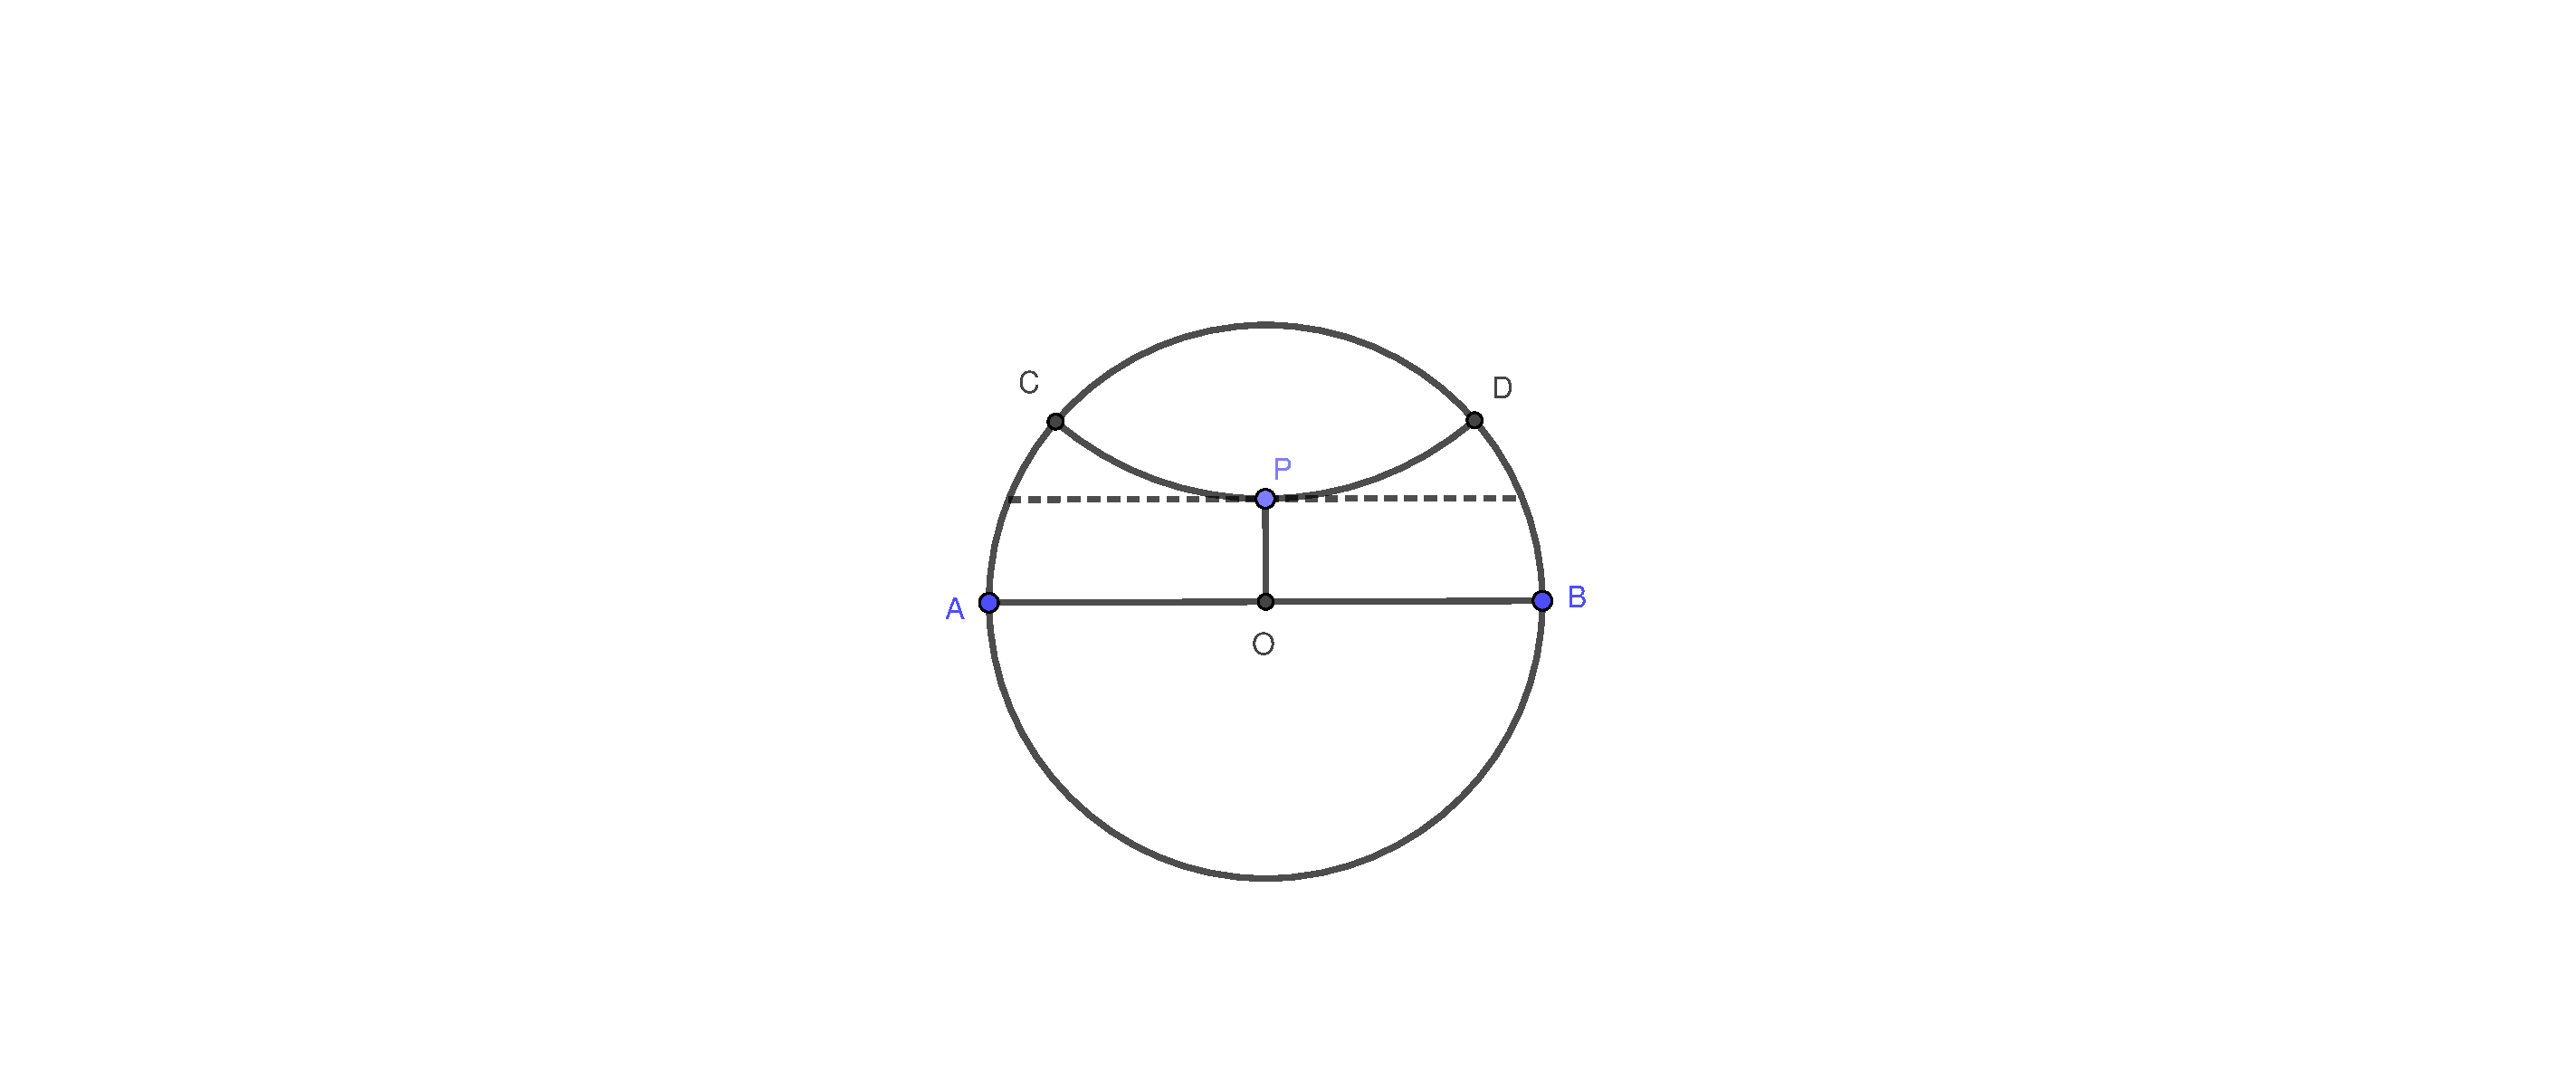
\includegraphics[width=\textwidth]{Duong_song_song_phan_ky.pdf}
\end{figure}

\begin{figure}[ht]
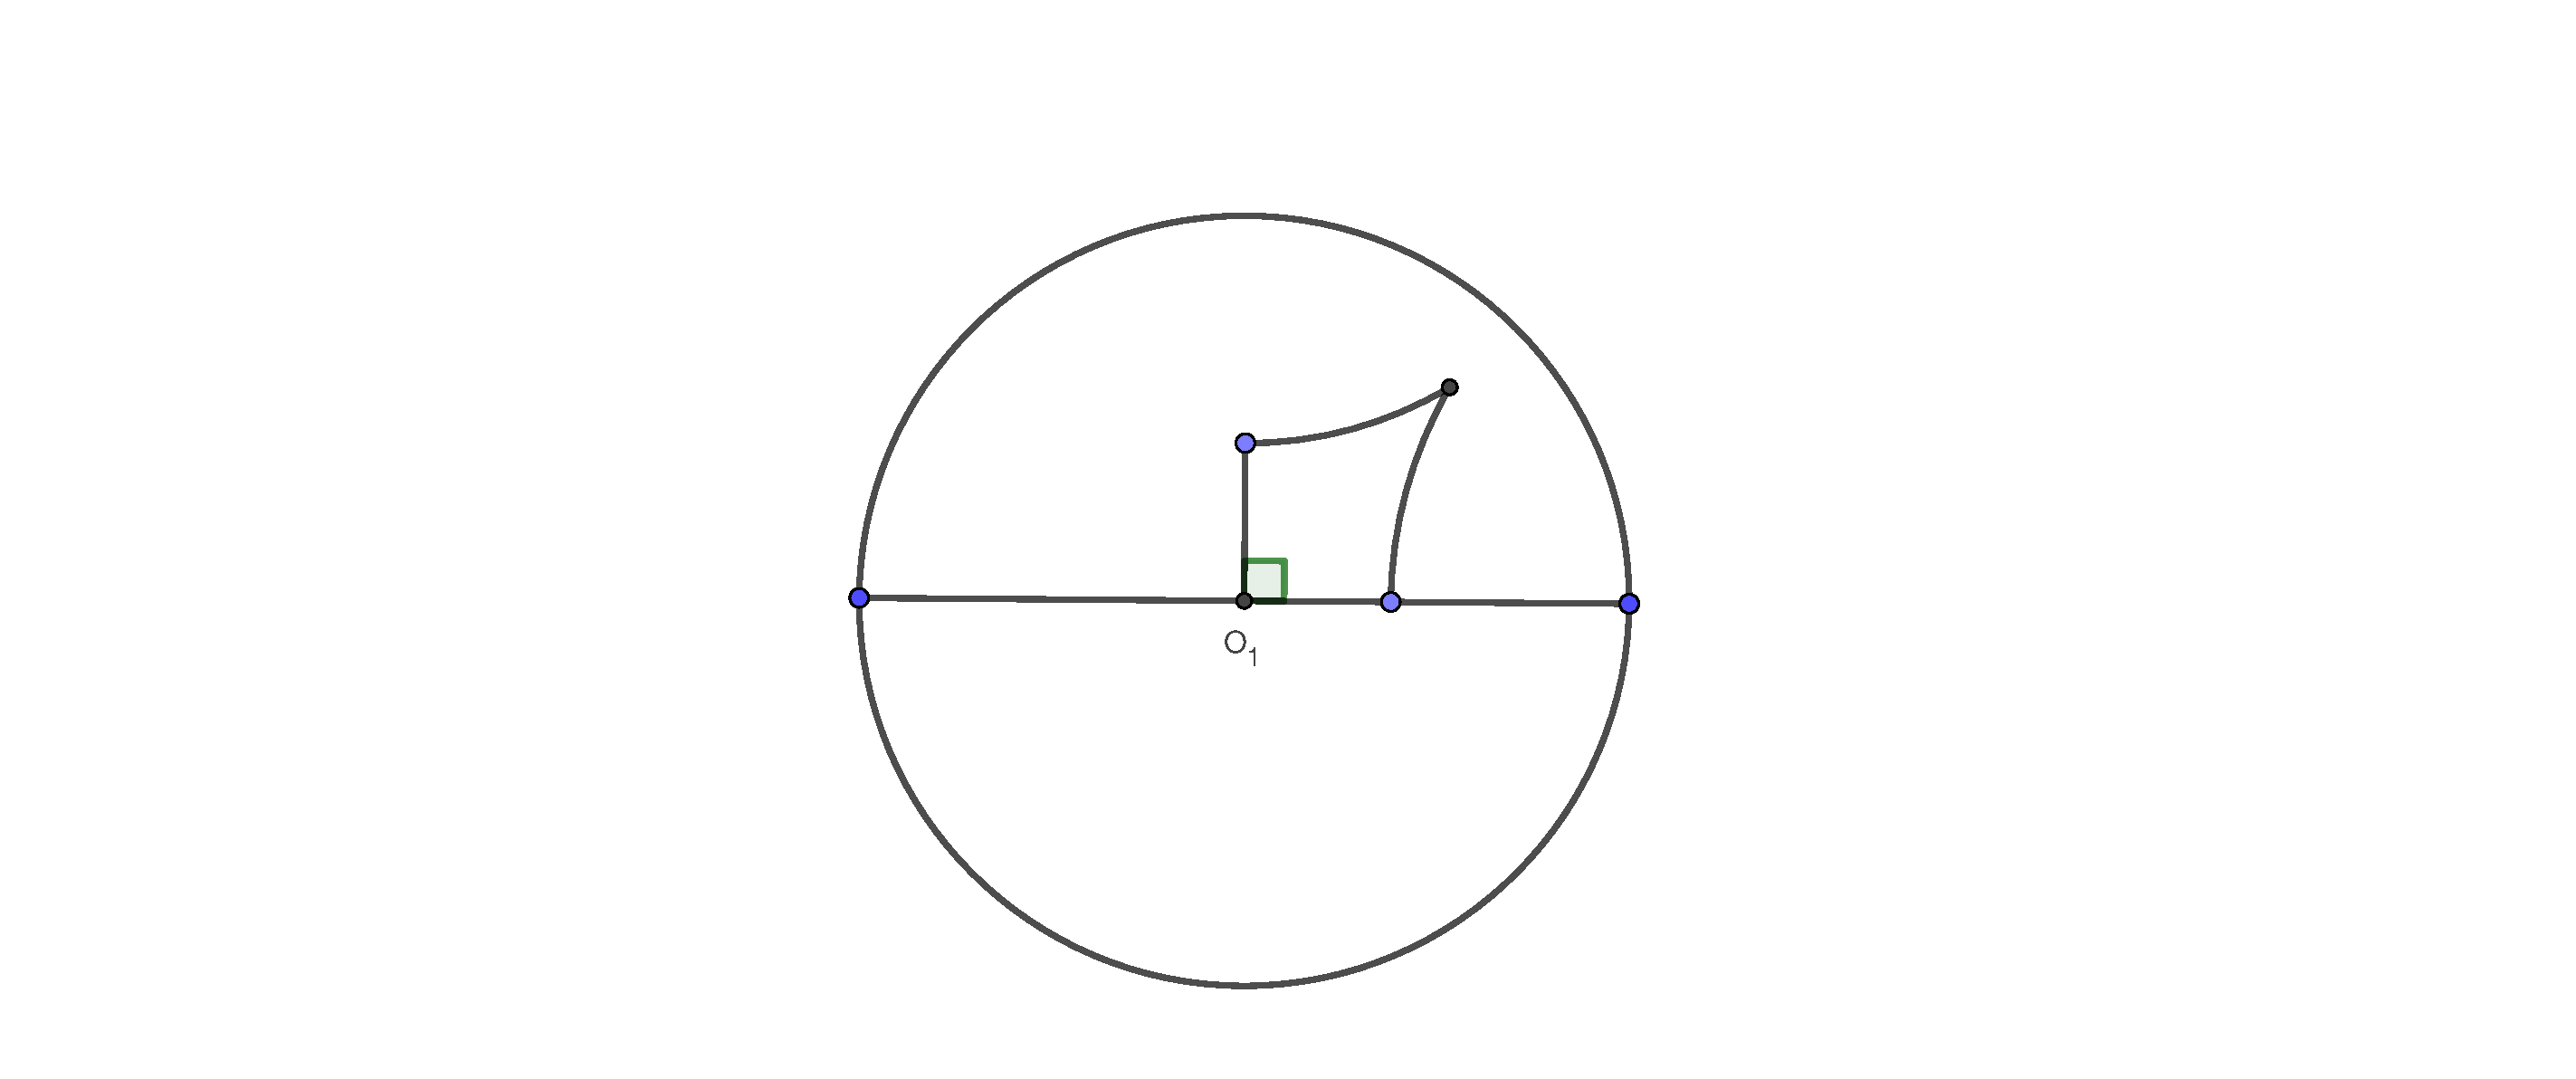
\includegraphics[width=\textwidth]{Tu_giac_Lambert.pdf}
\end{figure}

\begin{figure}[ht]
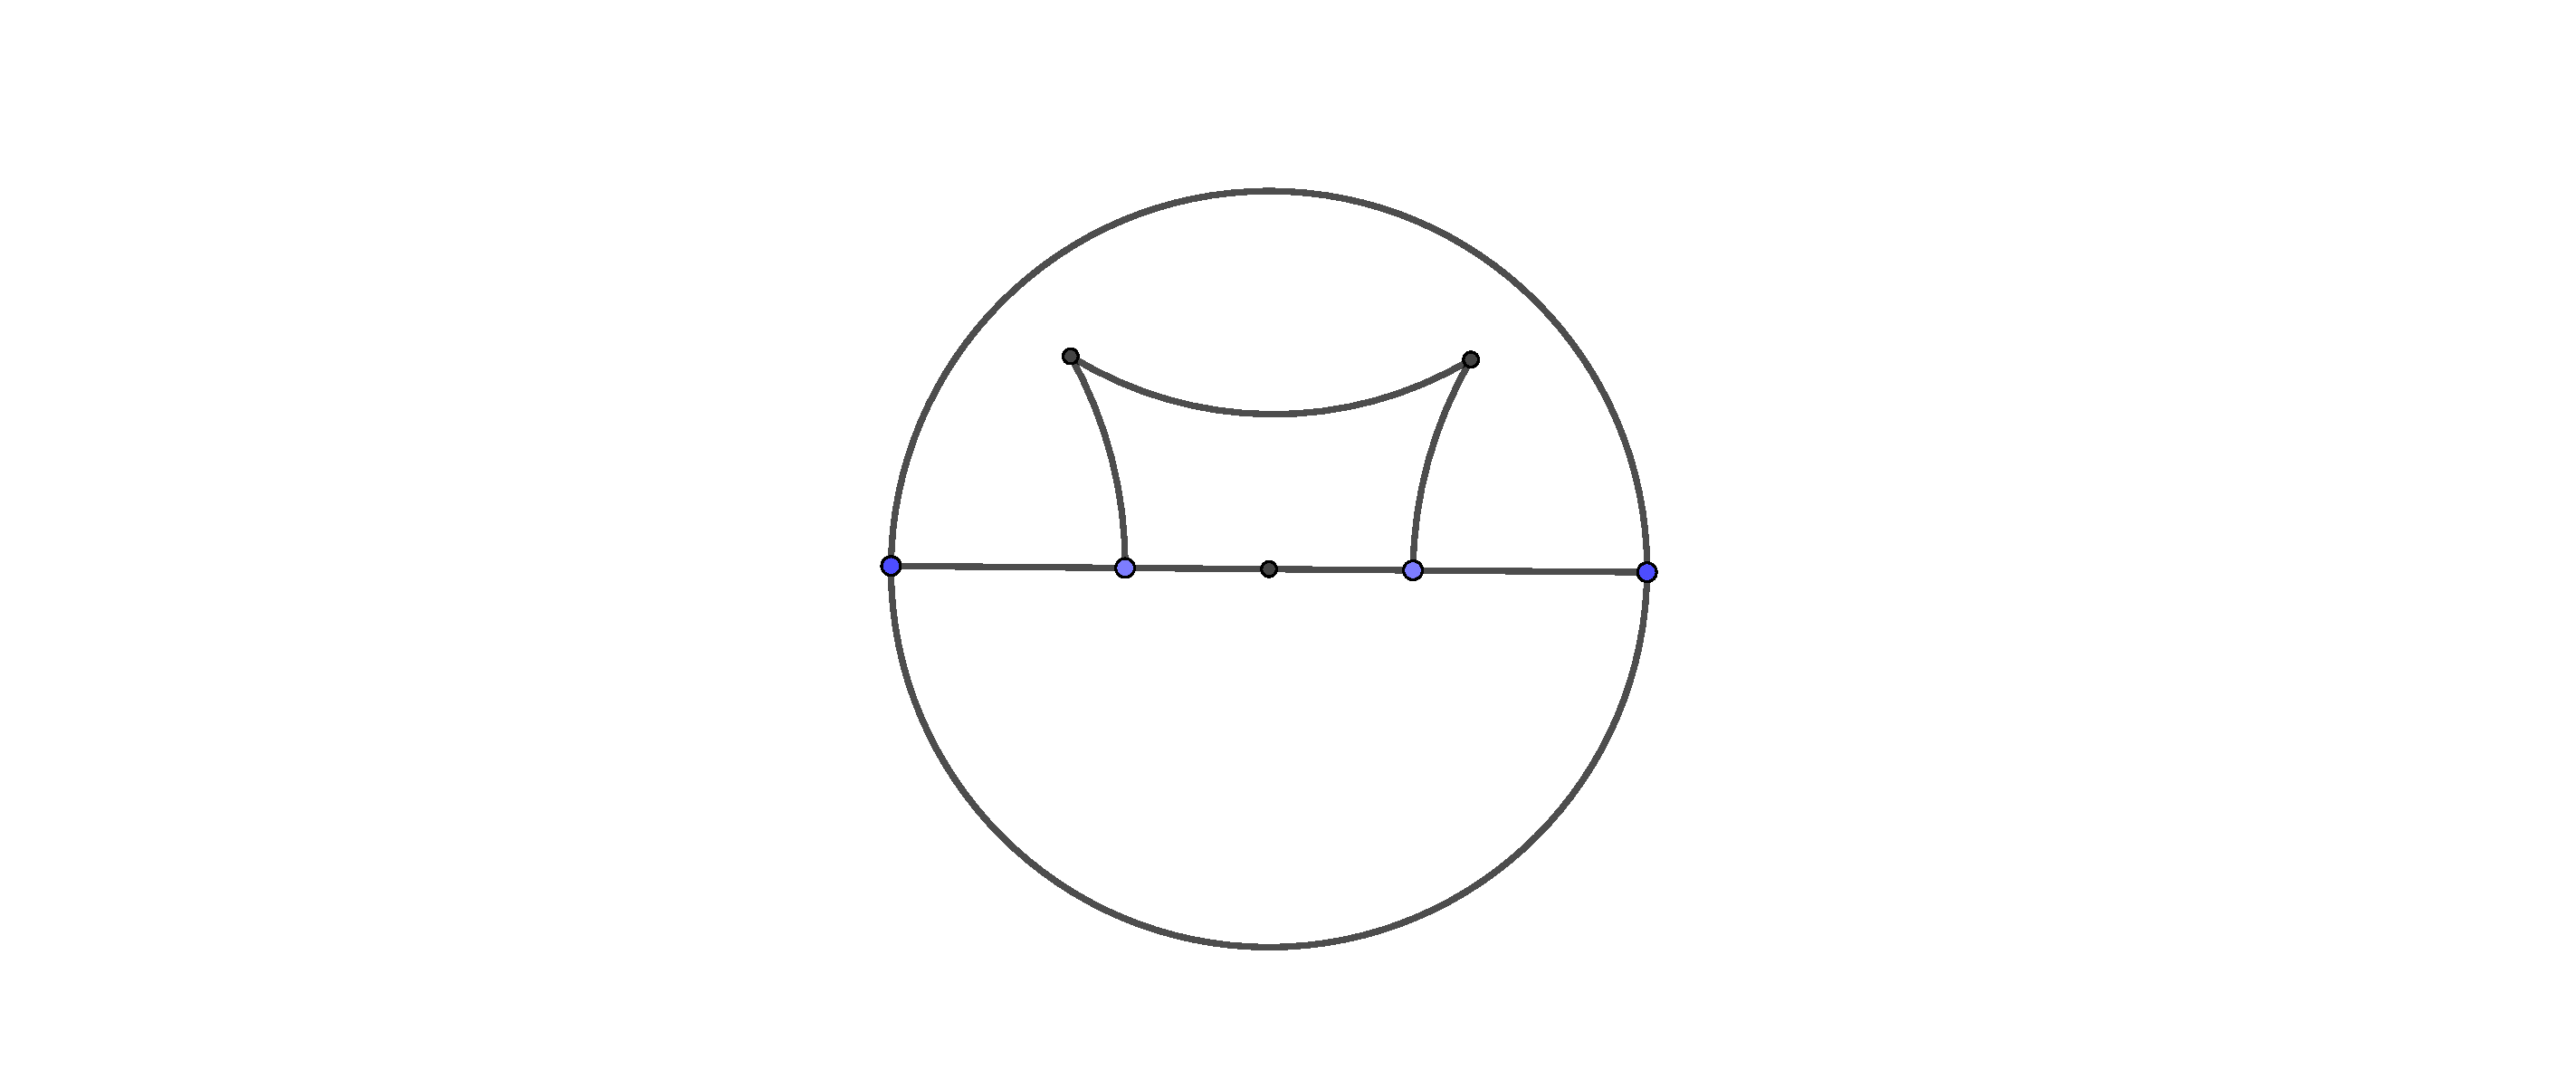
\includegraphics[width=\textwidth]{Tu_giac_Saccheri.pdf}
\end{figure}	
	
	
	
	\begin{figure}[H]
		\vspace*{-5pt}
		\centering
		\captionsetup{labelformat= empty, justification=centering}
		\includegraphics[width= 0.9\linewidth]{Đường song song giới hạn Poincare.pdf}
		\includegraphics[width= 0.9\linewidth]{Đường song song phân kỳ.pdf}
		\includegraphics[width= 0.9\linewidth]{Tứ giác Lambert.pdf}
		\includegraphics[width= 0.9\linewidth]{Tứ giác Saccheri.pdf}
%		\caption{\small\textit{\color{}}}
		\vspace*{-10pt}
	\end{figure}	
	Lưu ý nhỏ trước khi đi tiếp: ta có thể chứng minh được rằng mọi mô hình của hình hyperbolic đều là ``đẳng cấu''. Nôm na điều đó nghĩa là hai mô hình có cấu trúc tương đồng, còn cụ thể là sẽ tồn tại một quy tắc ghép đôi $1-1$ các điểm và đường thẳng từ mô hình này sang mô hình khác sao cho các quan hệ ``nằm trên'', ``đi qua'', ``nằm giữa'' và ``bằng nhau'' được bảo toàn. Ta sẽ gián tiếp định nghĩa quan hệ ``bằng nhau'' trong mô hình Beltrami--Klein nhờ vào mô hình Poincaré, đồng thời cũng sẽ có chứng minh cho các tiên đề về các quan hệ ``nằm trên'', ``đi qua'', ``nằm giữa'', và tiên đề Dedekind trong mô hình Poincaré, bởi các kết quả đó có thể được dễ dàng kiểm chứng ở mô hình Beltrami--Klein và lại có phép đẳng cấu trên. Một trong những phép đẳng cấu như vậy có nội dung như sau:
	

\begin{figure}[ht]
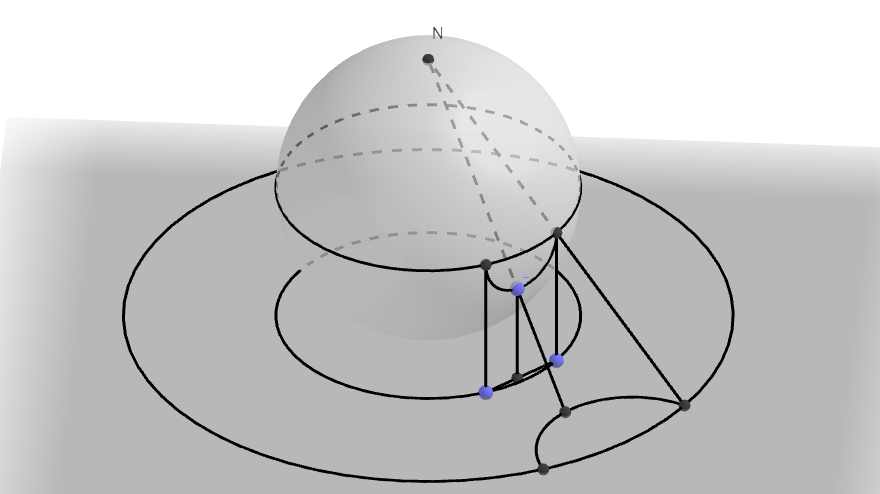
\includegraphics[width=\textwidth]{Klein_sang_Poincare.png}
\end{figure}

Dựng một mặt cầu tiếp xúc với mặt phẳng chứa đường tròn $\gamma$ của mô hình Beltrami-Klein tại tâm đường tròn. Để chuyển đổi từ mô hình Klein sang mô hình Poincar\'e, ta chiếu vuông góc dây mở trong mô hình Klein lên mặt cầu. Từ điểm N trên đỉnh mặt cầu, với mỗi điểm M trên hình chiếu vuông góc của dây mở lên mặt cầu, ta chiếu xuyên tâm N để đưa M trở lại mặt phẳng chứa $\gamma$ thành điểm M’ là giao điểm của đường NM với mặt phẳng ấy. Khi này một dây mở của mô hình Klein sẽ trở thành một đường Poincar\'e trong đường tròn đồng tâm và bán kính gấp đôi $\gamma$. Ta vị tự tâm O tỷ số $1/2$  là đưa đường tròn mới về $\gamma$.

Tiếp theo là định nghĩa độ dài đoạn trong mô hình Poincar\'e:

\textbf{Định nghĩa1.}  Với hai điểm A, B nằm bên trong đường tròn gamma và M, N là hai ``giao điểm” của đường Poincar\'e đi qua A, B với gamma. Khi ấy độ dài trong mô hình Poincar\'e của đoạn AB là:
\[ d(AB) = |\ln{(AB, MN)}| \]
Định nghĩa của tỷ số kép cho bộ 4 điểm cùng nằm trên một đường thẳng/ đường tròn đã được nêu ở phần trên. Không khó để chỉ ra là tỷ số kép này là số thực dương, do A, B nằm bên trong đường tròn $\gamma$. Đừng để ký hiệu logarit thêm vào làm cho hoang mang, nó ở đó chỉ để biến tính nhân thành tính cộng, điều này sẽ rõ trong chứng minh. Giá trị tuyệt đối được thêm vào để bất kể thứ tự của P và Q, của A và B, độ dài ko đổi dấu sang âm.

Ta định nghĩa đoạn AB bằng đoạn CD trong hình hyperbolic nếu như d(AB) = d(CD). Không khó có được rằng quan hệ bằng nhau có tính bắc cầu, và một đoạn bằng chính nó.
Cố định 1 điểm A trên đường Poincar\'e có hai đầu là M và N, để điểm B chạy liên tục từ A tới M sao cho thứ tự các điểm là N, A, B, M như hình. tỷ số kép (AB, MN) sẽ tăng liên tục từ 1 đến dương vô cùng, do $\frac{AM}{AN}$ cố định, BM tiến tới 0 và BN tiến tới MN. Cố định B và cho A chạy liên tục từ B tới N cũng tương tự. Do chạy liên tục nên tỷ số kép trên có thể nhận mọi giá trị lớn hơn hoặc bằng 1, ta chứng minh được rằng: với một đoạn cho trước và một tia nào đó, lấy được một điểm cách gốc tia đó dài bằng đoạn kia

\begin{figure}[ht]
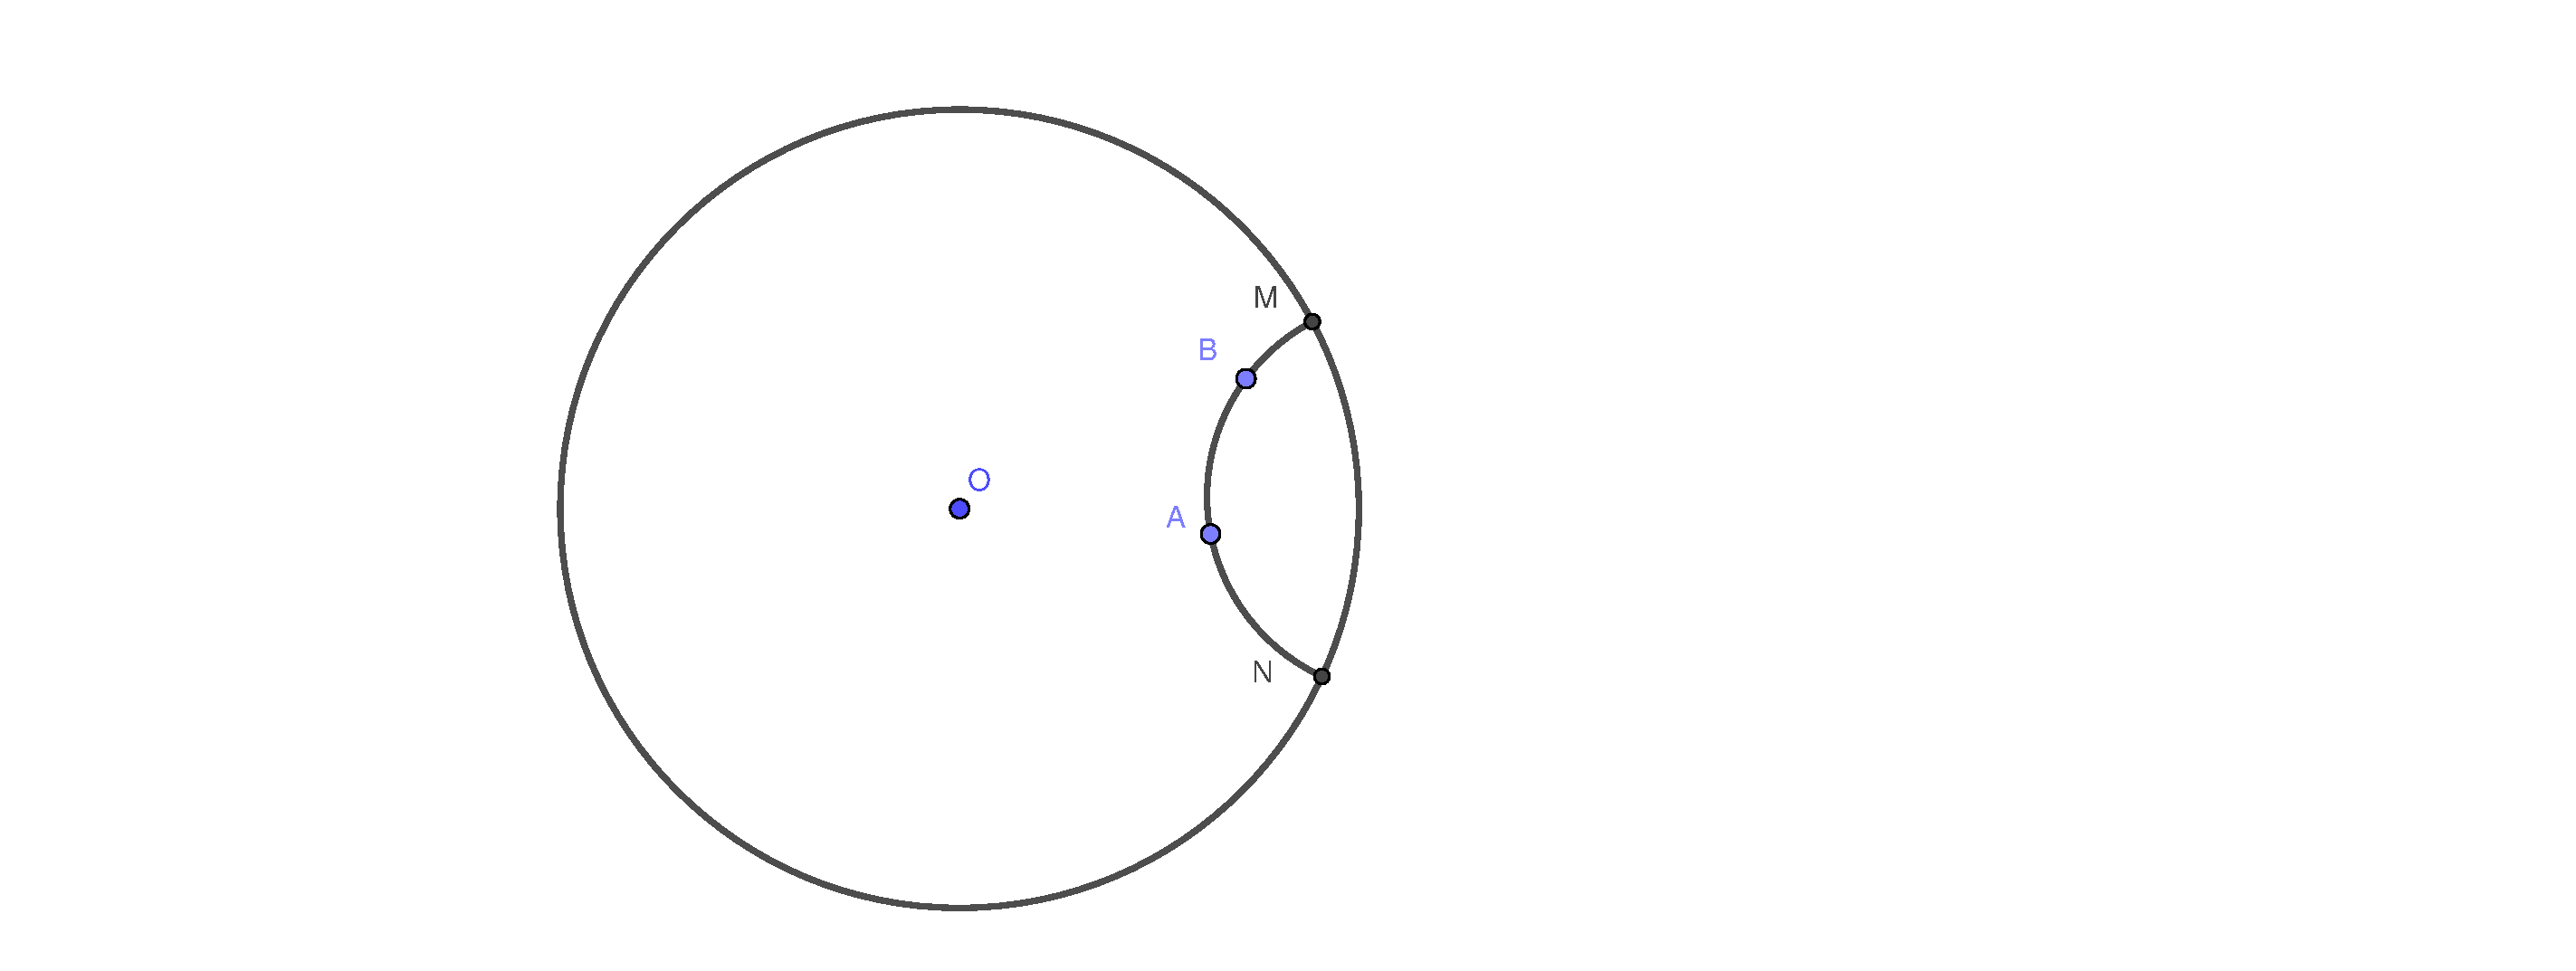
\includegraphics[width=\textwidth]{Tiende_NTDQ_1.pdf}
\end{figure}

Ta sẽ được phép cộng trừ cạnh thoải mái một khi chứng minh được là với điểm C nằm giữa A và B (trong mô hình Poincar\'e) thì d(AC) + d(CB) = d(AB). Lấy hai đầu M, N của đường Poincar\'e qua A và B để thứ tự các điểm là N - A - C - B - M.
Khi ấy các tỷ số kép sắp được đề cập đều lớn hơn 1 và ta có thể bỏ dấu giá trị tuyệt đối. Lúc này:
\begin{eqnarray*}
d(AC) + d(CB)& =& \ln{(AC, MN)} + \ln{(CB, MN)}\\
& =& \ln{\left(\frac{MA}{MC} : \frac{NA}{NC} . \frac{MC}{MB} : \frac{NC}{NB} \right)}\\
& =& \ln{ \left(\frac{MA}{MB} : \frac{NA}{NB}\right)}\\
& =& \ln{(AB, MN)} = d(AB),\end{eqnarray*}
chính là điều ta cần.

Về phần các tiên đề về sự bằng nhau của góc, ta cần nói qua về phép nghịch đảo và các tính chất liên quan tới hai đường tròn trực giao.

\section{Mở rộng của định nghĩa góc. Sơ lược về phép nghịch đảo}
Trước tiên ta mở rộng khái niệm góc trong hình Euclid. Có các trường hợp sau đây:
Đường thẳng d với đường tròn $\omega$: nếu chúng không có giao điểm thì sẽ không tạo góc với nhau. Nếu có giao điểm X, thì góc giữa d và $\omega$ được định nghĩa là góc giữa d và tiếp tuyến của $\omega$ tại X.
Giữa hai đường tròn $(O_1)$ và $(O_2)$, hay giữa hai đường cong có tiếp tuyến tại giao điểm: nếu chúng có giao điểm là Y thì góc giữa chúng là góc giữa hai tiếp tuyến của chúng tại Y. Đặc biệt nếu góc ấy là góc vuông thì ta gọi hai đường tròn là trực giao. Định nghĩa này phù hợp với định nghĩa ta đưa ra lúc trước. 

Phần bên dưới sẽ là giới thiệu về phép nghịch đảo. Những độc giả đã quen thuộc với phép biến hình này có thể bỏ qua. 

Phép nghịch đảo là một phép biến hình trong hình học Euclid, được ghi nhận lần đầu tiên trong công trình của Apollonius xứ Perga, thuộc Hy Lạp cổ đại, và được phát triển sâu hơn bởi nhiều người khác.
 
Với một điểm O và số thực k khác 0 bất kỳ, ta định nghĩa phép nghịch đảo tâm O, phương tích k là phép biến mỗi điểm Q khác O trên mặt phẳng thành điểm Q’ sao cho Q’ nằm trên đường thẳng đi qua O, Q, và 
$ \overline{OQ}\cdot \overline{OQ’} = k$. 
Nói chung ta cũng ký hiệu Q’ là ảnh của điểm Q qua phép nghịch đảo ta đang xét trong văn cảnh.
Phép nghịch đảo qua đường tròn tâm O bán kính R được định nghĩa là phép nghịch đảo tâm O phương tích $R^2$.

Khi một điểm P dịch chuyển gần lại về tâm nghịch đảo O theo phương một đường thẳng nào đó, ảnh P’ sẽ dịch chuyển xa khỏi O cũng theo phương đó. Vì thế một số người quy ước ảnh của điểm O qua phép nghịch đảo là ``điểm vô cùng”. Tuy nhiên bởi phương đường thẳng này là chọn tùy ý nên ``điểm vô cùng” này sẽ khác O và nằm trên mọi đường thẳng đi qua O, vì thế sẽ khác so với các điểm vô cùng trong mặt phẳng xạ ảnh. Ở đây chúng ta sẽ không xét đến ảnh của điểm O để đỡ phức tạp, một vài kết quả trong phần khảo sát ảnh sẽ hơi khác so với những gì độc giả có thể đã quen biết.
 
Sau đây là một số tính chất có thể được dễ dàng suy ra từ định nghĩa và xét các tam giác đồng dạng theo trường hợp c-g-c:

- Phép nghịch đảo là một involution(tự nghịch/ đối hợp), tức là tác động cùng một phép nghịch đảo hai lần thì trở về trạng thái ban đầu (hợp hai lần của một phép nghịch đảo là phép đồng nhất). Nói cách khác thì một phép nghịch đảo có hàm ngược là chính nó.
Tổng quát hơn thì hợp của hai phép nghịch đảo cùng tâm là một phép vị tự tâm đó \\
- Tập hợp tất cả các điểm bất động qua phép này là đường tròn nghịch đảo. \\
- Cách dựng ảnh của một điểm qua phép nghịch đảo đường tròn:

    +) P nằm trong đường tròn: vẽ dây TU đi qua P và vuông góc OP, P’ chính là giao điểm của hai tiếp tuyến tại U và T của (O, R)\\
    +) P nằm ngoài đường tròn: vẽ 2 tiếp tuyến PT, PU tới đường tròn. P’ = TU cắt OP \\
- Phép nghịch đảo biến P thành P’, Q thành Q’, và O, P, Q không thẳng hàng, thì $\Delta  P’OQ’ \sim  \Delta POQ$ \\
- $A’B’ = |k|. \frac{AB}{OA.OB}$ \\
- Ảnh của một đường tròn trực giao với đường tròn nghịch đảo là chính nó.

\begin{figure}[ht]
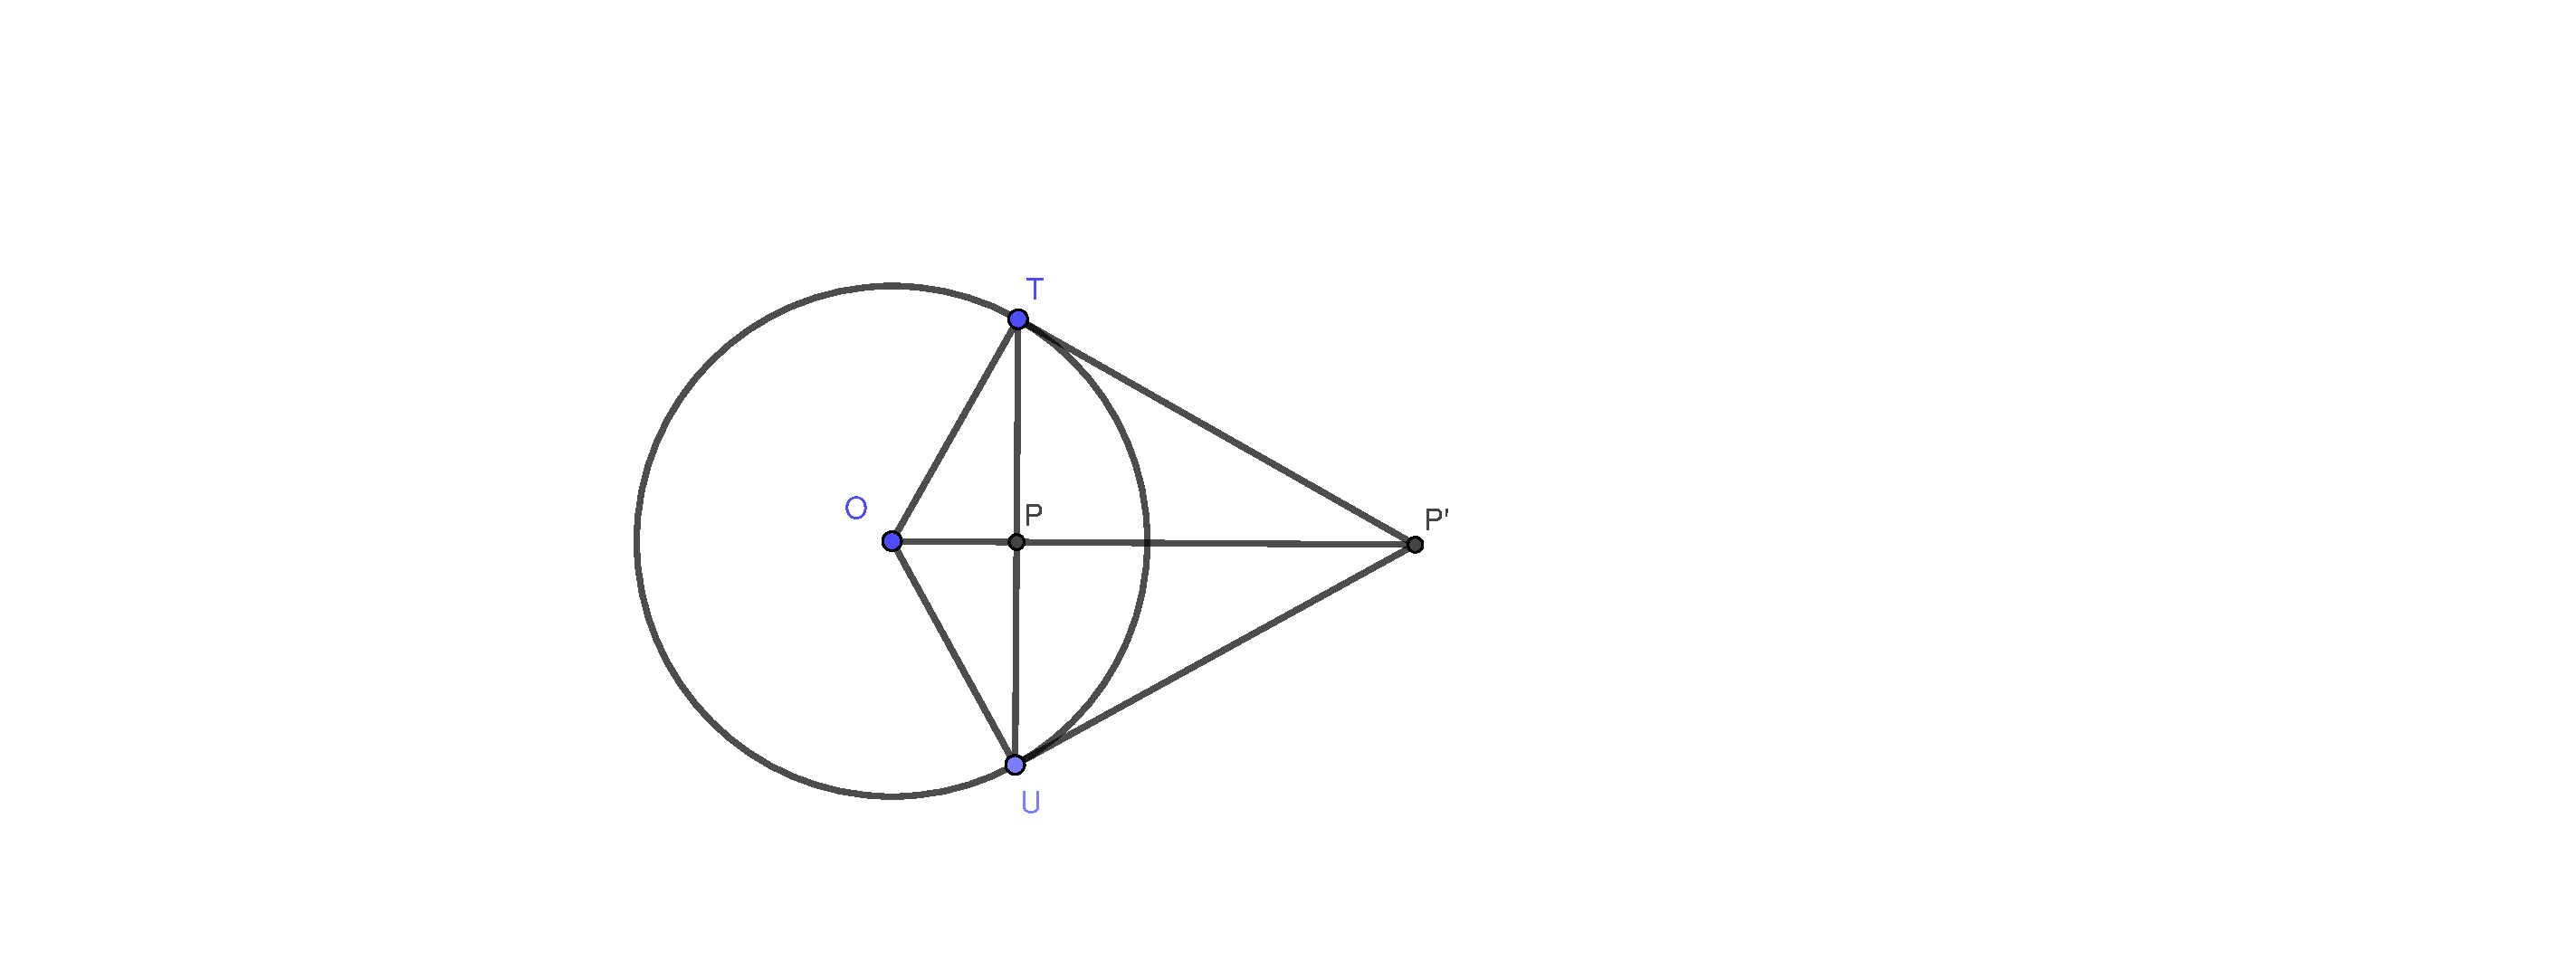
\includegraphics[width=\textwidth]{Dung_anh_phep_nghich_dao.pdf}
\end{figure}

Tiếp theo ta sẽ tìm hiểu hình dạng ảnh của đường thẳng và đường tròn qua phép nghịch đảo đường tròn. Vẫn xét phép nghịch đảo qua (O, R) như trên: \\
- Một đường thẳng l đi qua O sẽ biến thành l \\
- Một đường thẳng l không đi qua O sẽ biến thành đường tròn đường kính OA’, với A là chân đường vuông góc từ O xuống l. \\ 
- Một đường tròn đi qua O sẽ biến thành đường thẳng l vuông góc với OA’ tại A’, trong đó OA là đường kính đường tròn trên. Do tính chất tự nghịch của phép nghịch đảo, điều này sẽ có ngay sau khi chứng minh tính chất thứ 2. \\
- Một đường tròn (O1) không đi qua O sẽ biến thành một đường tròn (O2) không đi qua O. O cũng là một tâm vị tự của hai đường tròn. 

Qua đây ta thấy phép nghịch đảo hầu như không bảo toàn hình dạng của đường thẳng và đường tròn, nhưng nó bảo toàn được hai đặc tính quan trọng khác là góc giữa hai hình và tỷ số kép của các bộ điểm. Thật vậy, phép nghịch đảo bảo toàn góc nhưng đảo ngược chiều của góc đó. Nó lại đồng thời bảo toàn các quan hệ nằm trên, đi qua, nằm giữa. Do đã có hệ thức về độ dài một đoạn qua phép nghịch đảo  $A’B’ = |k|. \frac{AB}{OA.OB}$ , ta sẽ chứng minh được là tỷ số kép bảo toàn qua phép biến hình này. Giờ đây việc mở rộng định nghĩa của tỷ số kép và góc cho các đối tượng phổ quát hơn tỏ rõ sự hữu dụng, khi mà hai đường thẳng qua phép nghịch đảo có thể biến thành một đường thẳng và một đường tròn, hoặc 2 đường tròn, bộ 4 điểm trên đường thẳng thì biến thành bộ 4 điểm trên đường tròn. Điểm thú vị là trong mô hình Poincar\'e, bảo toàn tỷ số kép dẫn đến bảo toàn độ dài Poincar\'e.

Sau đây là một tính chất quan trọng về đường tròn trực giao cùng với chứng minh., mà chúng tôi sẽ thực sự chứng minh:

\textbf{Định lý 2.} \textit{ Cho đường tròn (O, R) và điểm P khác tâm và không nằm trên đường tròn. Đường tròn (O’) đi qua P sẽ trực giao với (O) $ \leftrightarrow$ (O’) đi qua P’ - ảnh của P khi nghịch đảo qua (O).}

\begin{figure}[ht]
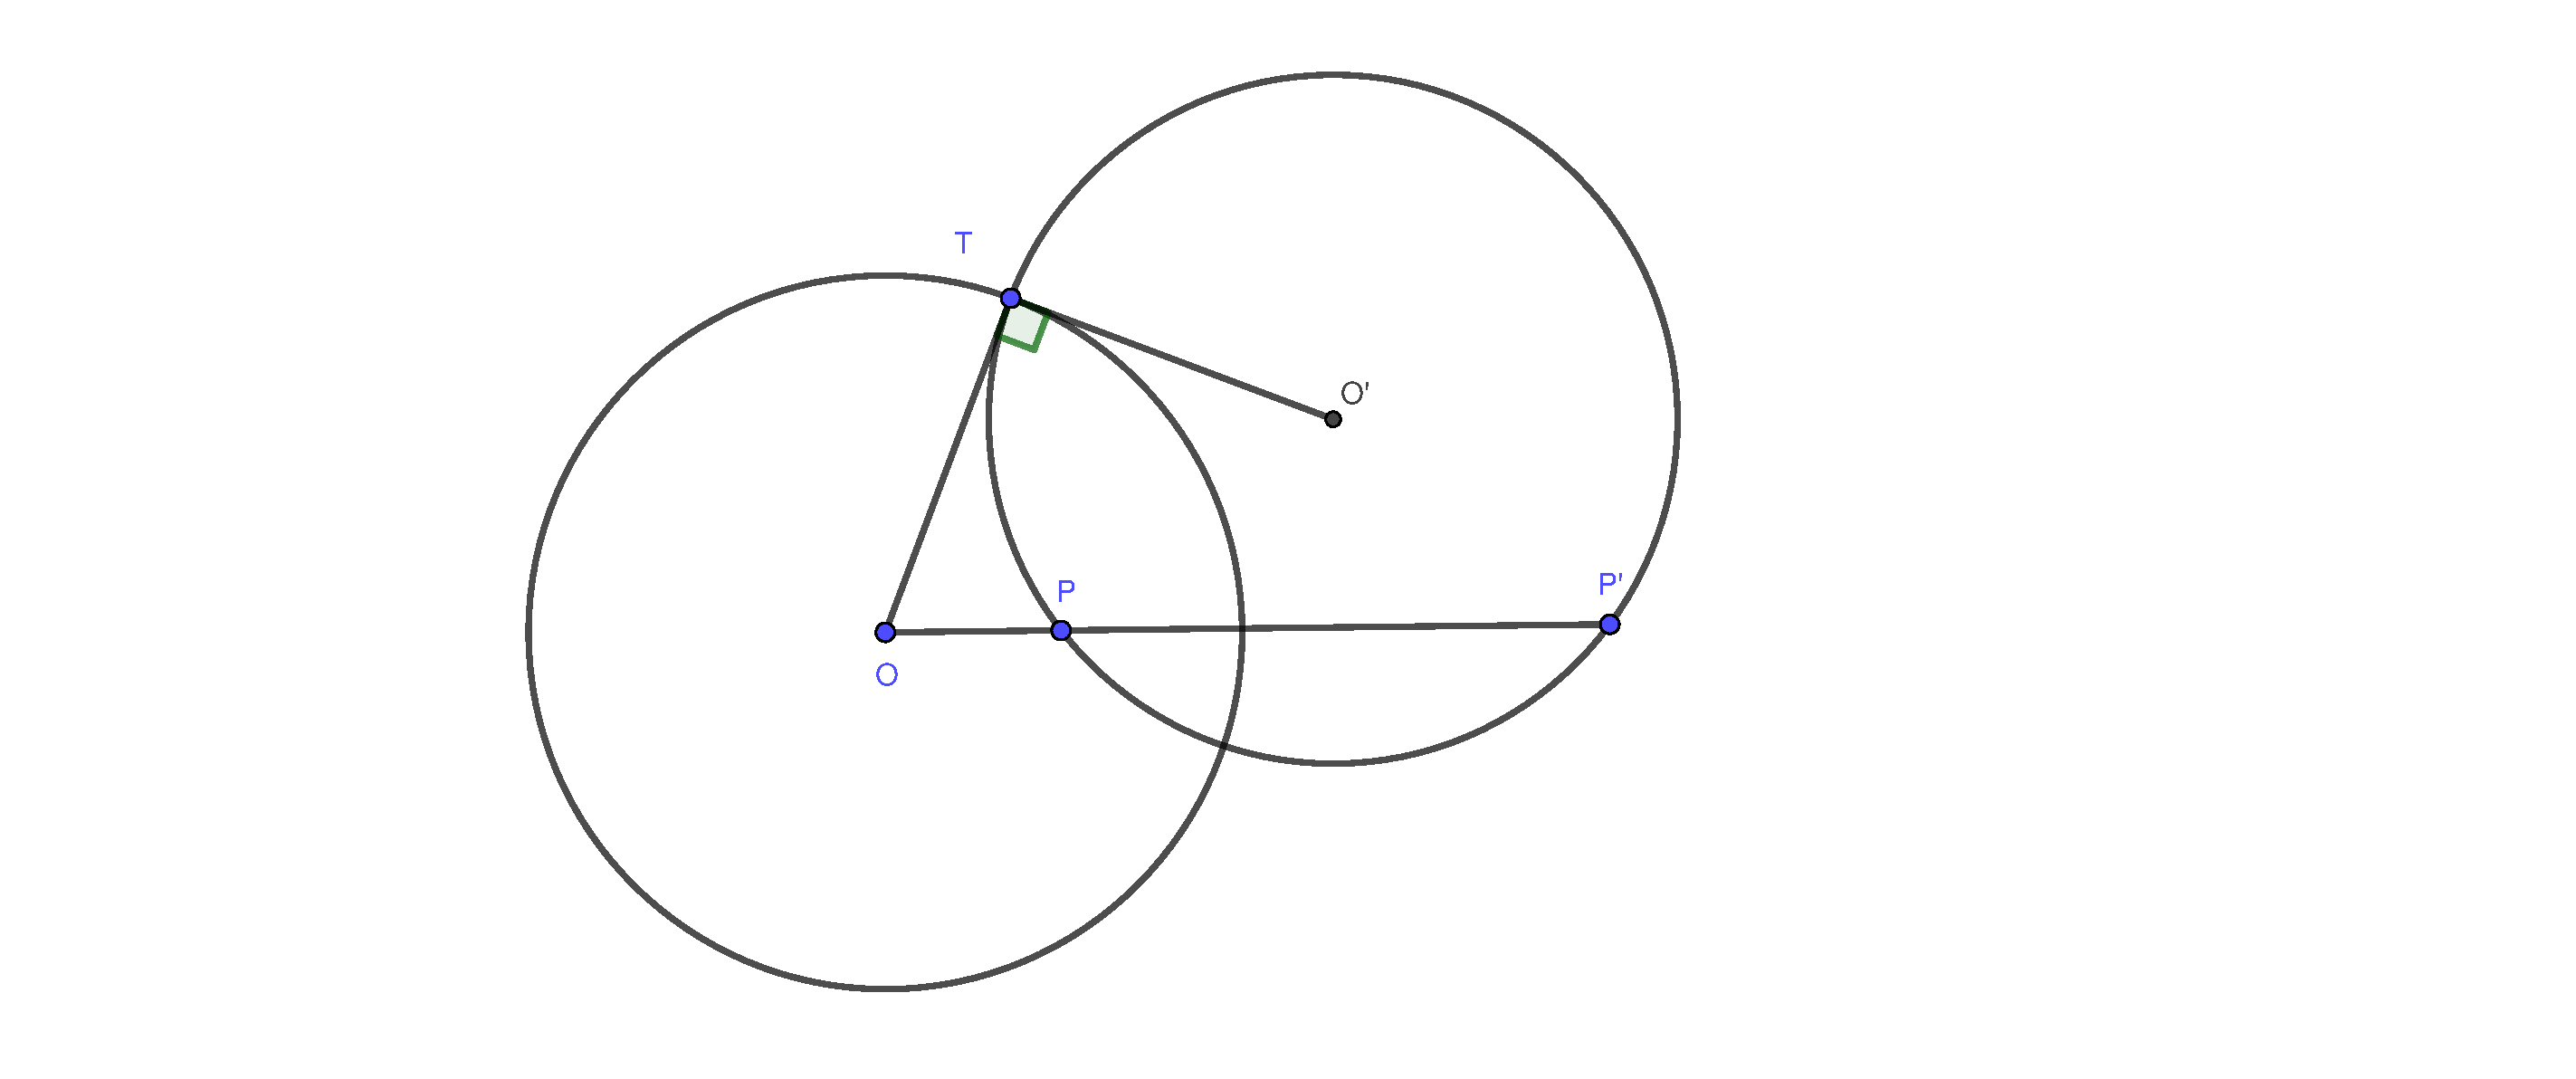
\includegraphics[width=\textwidth]{Dinh_ly_1.pdf}
\end{figure}


\textit{Chứng minh}. (Đảo) Giả sử (O’) đi qua P’, có ngay O’ thuộc trung trực PP’, từ việc P nằm giữa O, P’, ta suy ra được O’P<O’O, nghĩa là điểm O nằm ngoài (O’). Điều đó cho phép vẽ tiếp tuyến OT tới (O’), từ đó chứng minh được tg OPT đồng dạng tg OTP’. Từ tỷ lệ cạnh bằng nhau có là $OT^2 = OP.OP’ = R^2$ (định nghĩa nghịch đảo), tức T nằm trên (O, R). Lại có OTO’ là góc vuông, ta có được sự trực giao.

(Thuận) Gọi T, U là hai giao điểm của (O) và (O’) trực giao. Bởi hai tiếp tuyến tại T và U giao nhau tại O, O nằm ngoài (O’). Vậy nên OP cắt lại (O’) tại Q khác P, từ tam giác đồng dạng lại có $OP.OQ = OT^2 = R^2$ cho thấy Q là ảnh của P qua nghịch đảo (O, R).

\textbf{Hệ quả 3.} \textit{ Quỹ tích của tâm các đường tròn trực giao (O’) và đi qua P chính là trung trực PP’.
Đảo lại, với l nằm ngoài (O, R), hạ OO’ vuông góc l. (O’) trực giao (O) cắt OO’ tại điểm gọi là P. Khi ấy quỹ tích ở trên chính là l.}

Định lý này cho phép ta một các dựng đường Poincar\'e đi qua hai điểm M, N không thẳng hàng với tâm của $\gamma$ như sau. Vẽ M’ là ảnh nghịch đảo M qua $\gamma$, vẽ đường tròn qua ba điểm M, M’, N. Đường tròn ấy sẽ trực giao với $\gamma$ và ta có cung cần tìm. Do M, N xác định duy nhất, M’ cũng thế, và đường tròn qua 3 điểm này sẽ là duy nhất.

\section{Các tiên đề về sự bằng nhau}
Đã đến lúc chứng minh các tiên đề còn lại về quan hệ bằng nhau trong mô hình Poincar\'e đúng là định lý trong hình Euclid.

Vì góc được đo như ở hình Euclid nên nó cũng có tính chất bắc cầu và một góc bằng chính nó. Ta cần chỉ ra: với một góc cho trước và một tia AB thì dựng được C để $ \angle CAB$ bằng góc đó (các đối tượng ở đây hiểu theo nghĩa của mooh hình Poincar\'e). Nếu A trùng với tâm $ \gamma$ thì các đường Poincar\'e đi qua A chính là các dây mở, việc dựng sẽ như ở hình Euclid.
 Nếu không, bài toán quy về: cho trước một đường thẳng l đi qua A và không đi qua tâm O của $\gamma$, khi ấy có đúng một đường tròn (O’) trực giao với $\gamma$ và tiếp xúc với l tại A. Đường thẳng l này chính là đường tạo với tiếp tuyến của ``tia AB” góc bằng góc đề cho. 

Định lý ta vừa chứng minh cho thấy (O’) sẽ phải đi qua A’, do đó O’ nằm trên trung trực AA’. Mặt khác (O’) tiếp xúc l tại A, nên O’ nằm trên đường vuông góc với l tại A. Tóm lại, O’ sẽ được xác định duy nhất là giao điểm của hai đường kể trên.

Để sẵn sàng chứng minh trường hợp bằng nhau cgc của các tam giác Poincar\'e, ta cần hai bước đệm nữa:

\textbf{Định lý 4.} \textit{ Cho (O) trực giao (O’). Khi ấy, phép nghịch đảo qua (O') sẽ biến (O) thành (O) và biến phần bên trong (O) thành chính nó. Đồng thời phép này bảo toàn các quan hệ nằm trên, đi qua, nằm giữa và bằng nhau theo mô hình Poincar\'e. Ta gọi phép biến hình này là phép P-đối xứng với (O').
Tương tự với một đường thẳng d đi qua O,  d cũng gọi là trực giao với (O), và xét phép biến hình là đối xứng qua d. Phép này ta cũng gọi là phép P-đối xứng với d.}

\textbf{Định lý 5.} [về xây dựng phép P-đối xứng]  \textit{Với mỗi hai điểm A, B trong $\gamma$, tồn tại đường Poincar\'e $\delta$ sao cho phép P-đối xứng với $\delta$ biến A thành B. Giao điểm của đường Poincar\'e nối A và B với $\delta$ là trung điểm theo nghĩa Poincar\'e của AB. Trung điểm ở đây là điểm nằm trên đoạn và cách đều hai đầu mút.}

\textit{Chứng minh.} Xét các trường hợp:

- Hai điểm cách đều O. Chọn delta là đường kính mở của gamma vuông góc với đường thẳng (theo nghĩa Euclid) AB \\
- Một trong hai điểm trùng với O, giả sử là A. đường Poincar\'e đi qua A, B sẽ là đường kính mở qua OB. Chọn delta là (CC’), trong đó C là trung điểm OB theo nghĩa Poincar\'e. \\

\begin{figure}[ht]
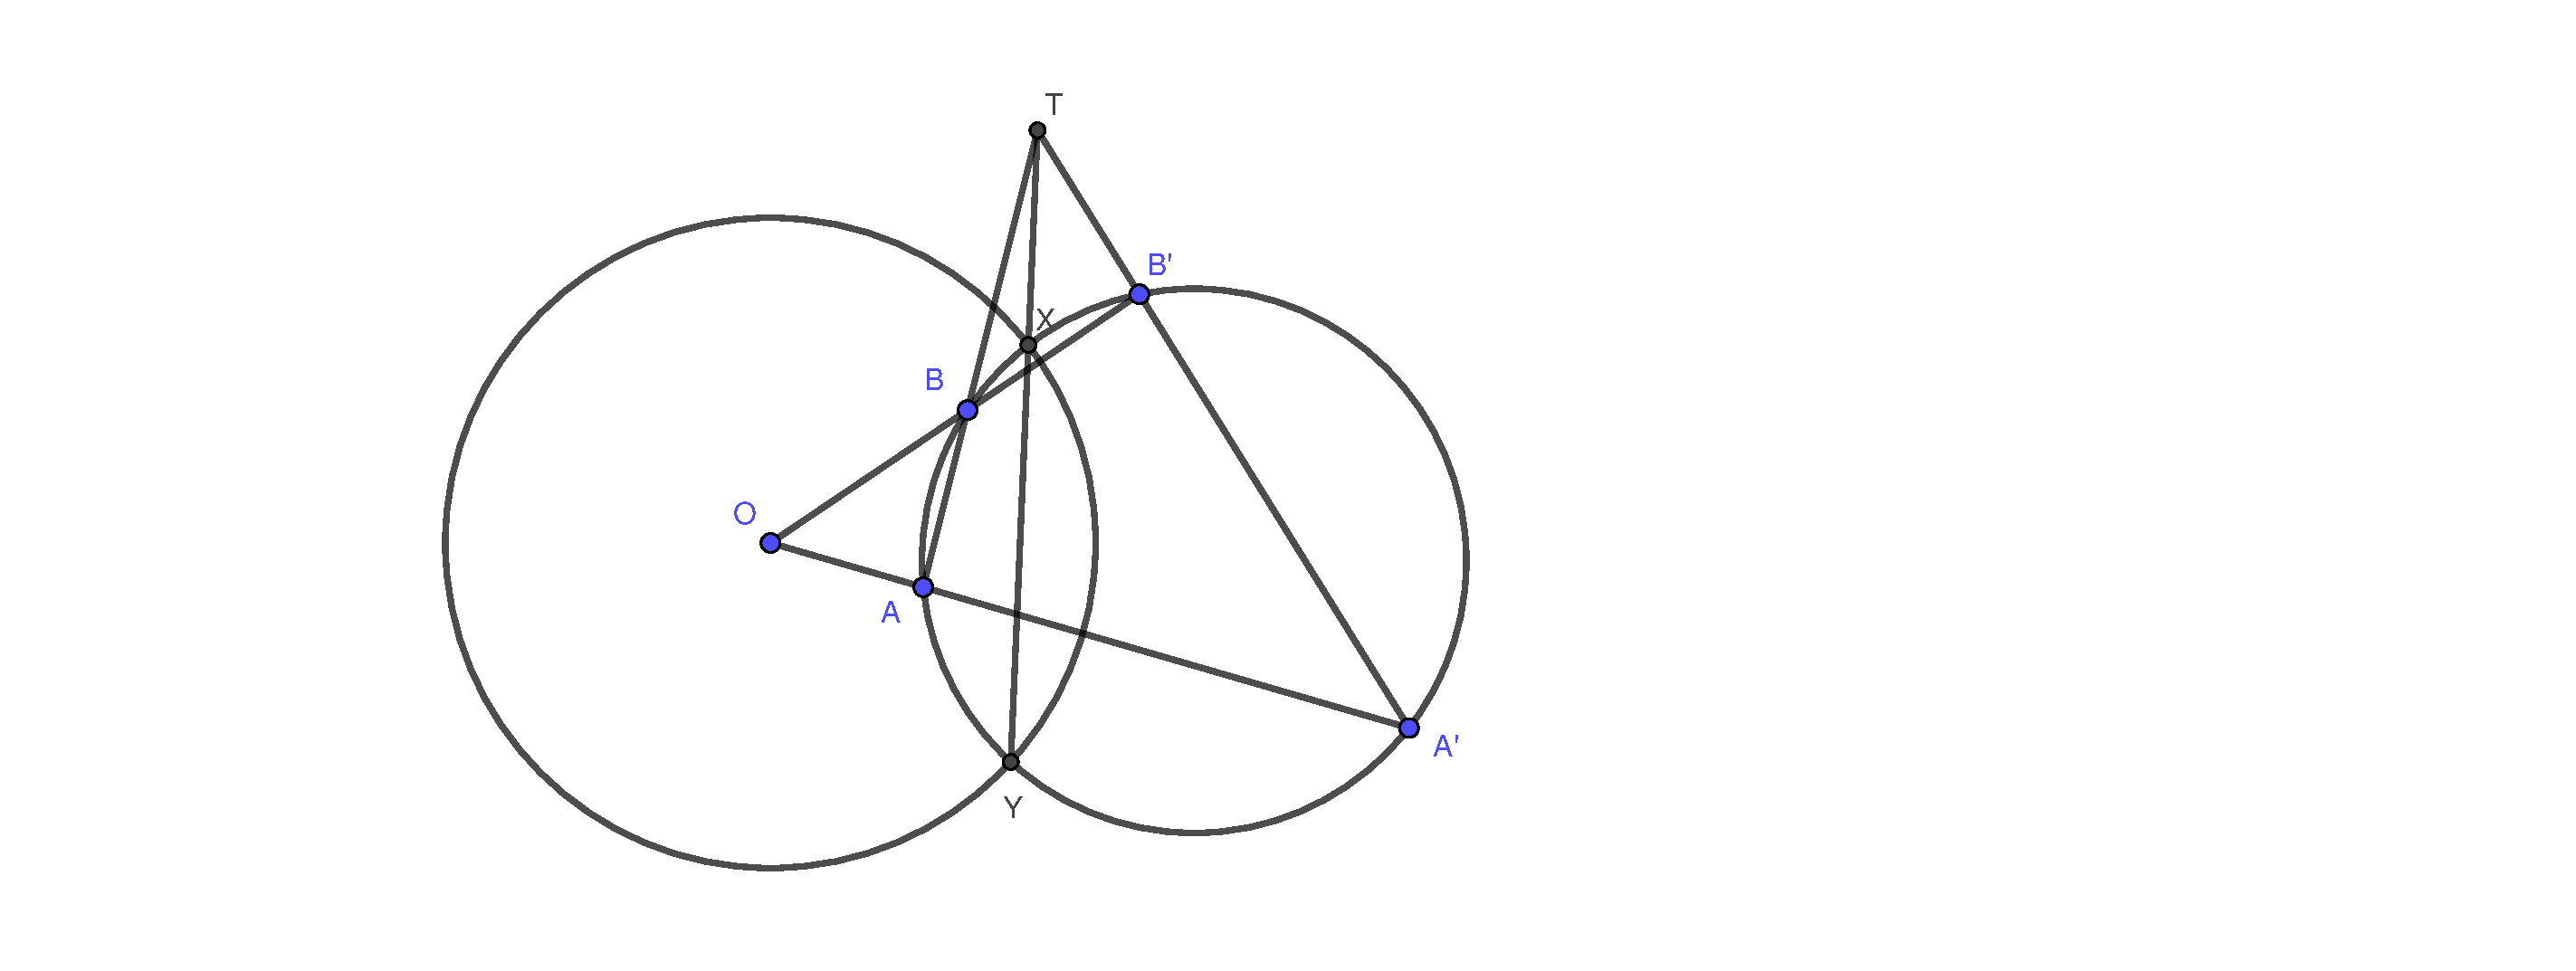
\includegraphics[width=\textwidth]{TH_3_dinh_ly_xay_dung.pdf}
\end{figure}

- A và B không nằm trên cùng một đường kính của $\gamma$. Gọi $\gamma$’ là đường Poincar\'e đi qua A và B, đây là một đường tròn trực giao với $\gamma$, gọi X, Y là giao điểm của $\gamma$’ và $\gamma$. Để ý rằng A’, B’ là giao điểm thứ hai của OA, OB với $\gamma$’. Gọi M, N là giao điểm của OA, OB với XY. Từ OX, OY là hai tiếp tuyến với gamma’, ta chỉ ra được (OM, AA’) = -1 = (ON, BB’), dẫn đến AB, A’B’ (có giao điểm do trường hợp 1 đã xét) và XY đồng quy tại điểm gọi là T. Chọn $\delta$ là $(T, \sqrt{TA.TB})$. \\

\begin{figure}[ht]
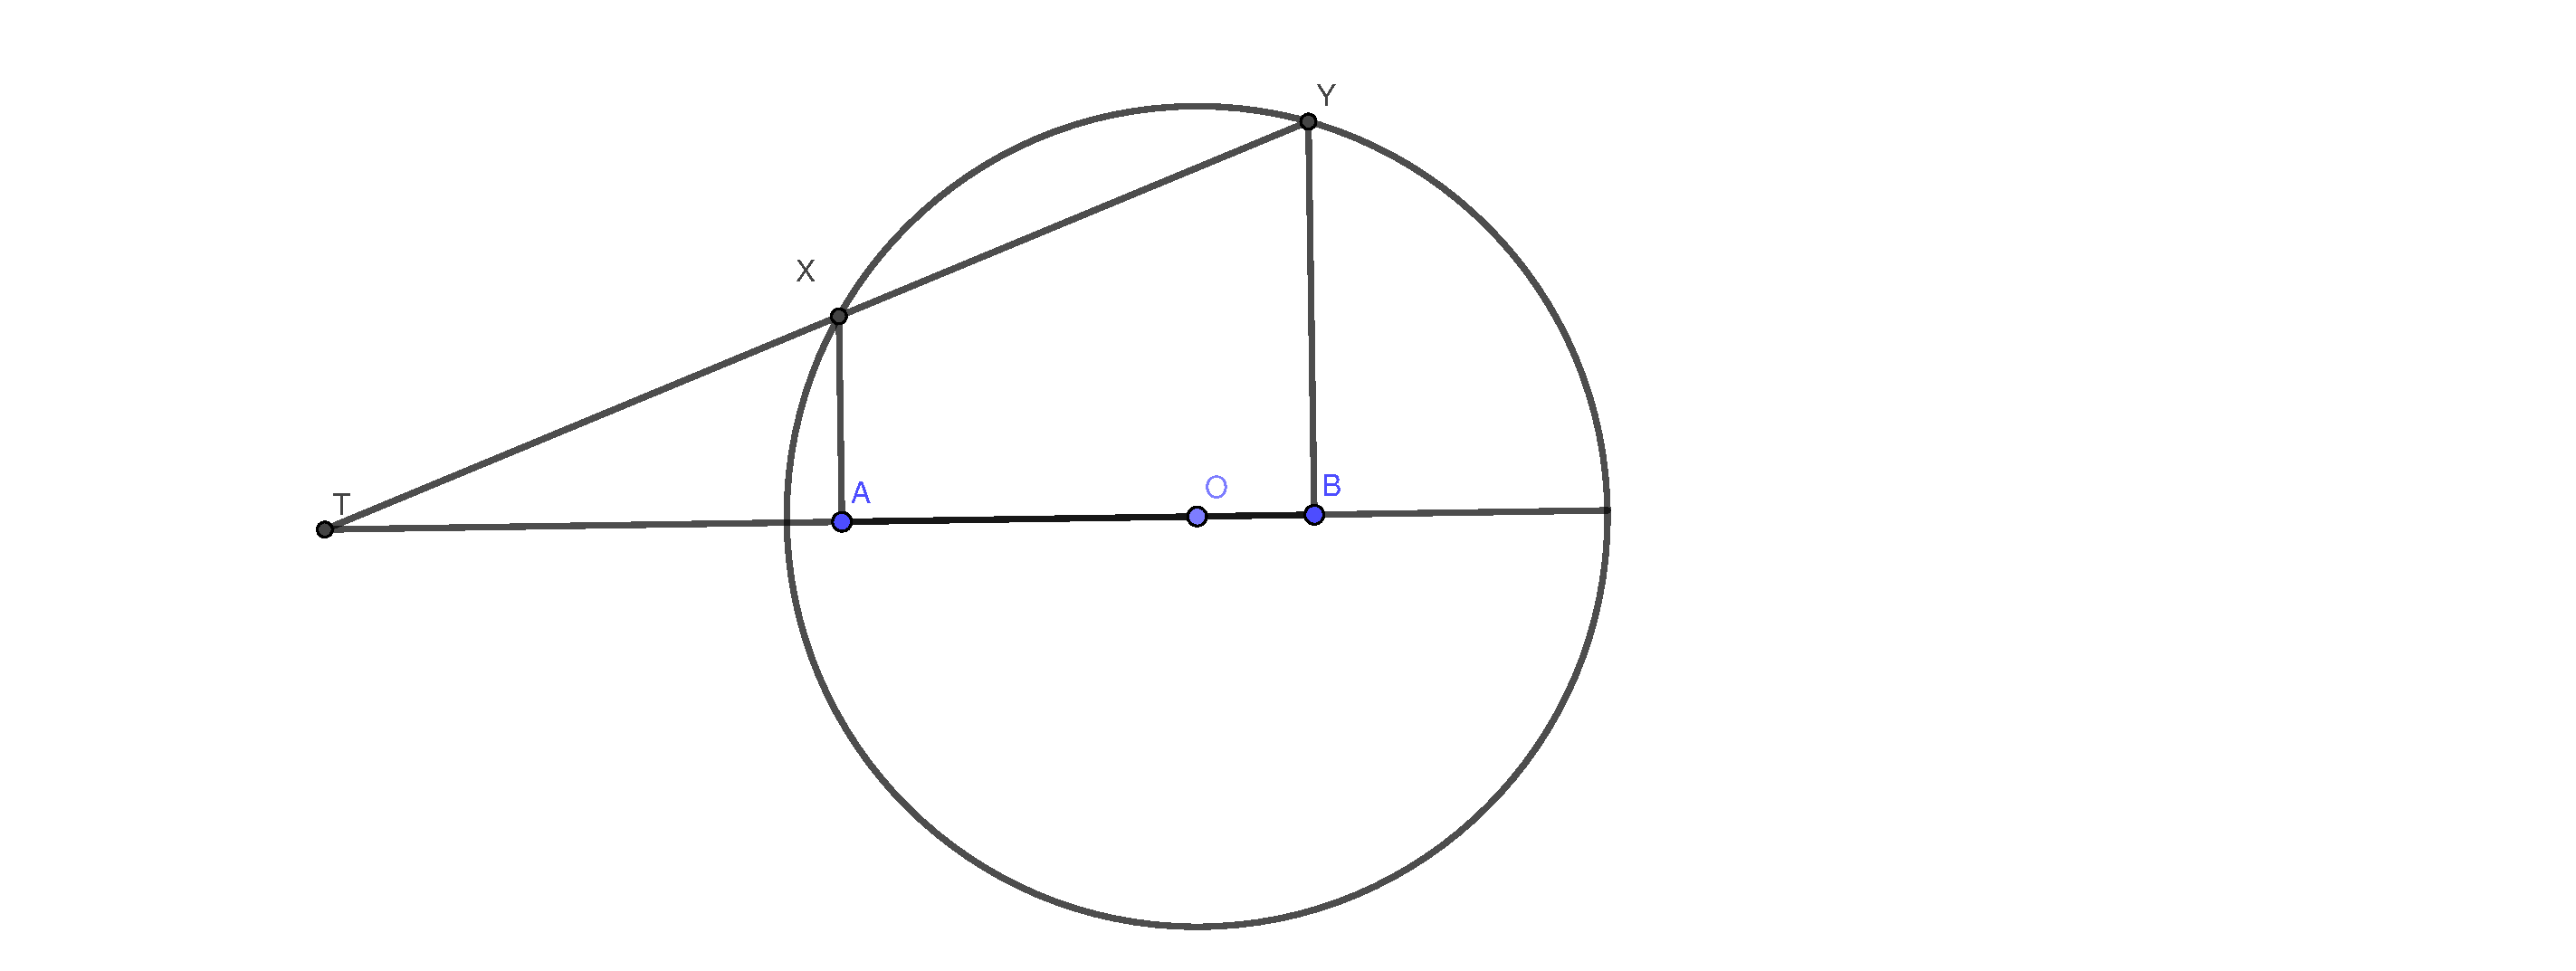
\includegraphics[width=\textwidth]{TH_4_dinh_ly_xay_dung.pdf}
\end{figure}

- A, B cùng nằm trên một đường kính XY của gamma và không cách đều O. Lấy 1 điểm D trên gamma sao cho DB vuông góc XY, gọi E là giao điểm thứ hai của (ABD) với gamma. E tổn tại vì hai đường tròn đã sẵn có điểm chung D, và chúng không thể tiếp xúc tại D do trung điểm AD không nằm trên OD. Gọi C là giao điểm của đường thẳng DE với XY, có CD.CE = CA.CB do ABDE là tứ giác nội tiếp. Chọn $\delta$ là $(C, \sqrt{CA.CB})$.

\section{Trường hợp bằng nhau cạnh-góc-cạnh}

Ta phát biểu lại trường hợp bằng nhau này.

\textbf{Định lý 8.}\textit{
Cho hai tam giác ABC và XYZ có: $ \angle A = \angle X, d(AB) = d(XY), d(AC) = d(XZ)$
Khi ấy hai tam giác này bằng nhau, nghĩa là $d(BC)  = d(YZ), \angle B = \angle Y, góc C = góc Z$.
}
\begin{figure}[ht]
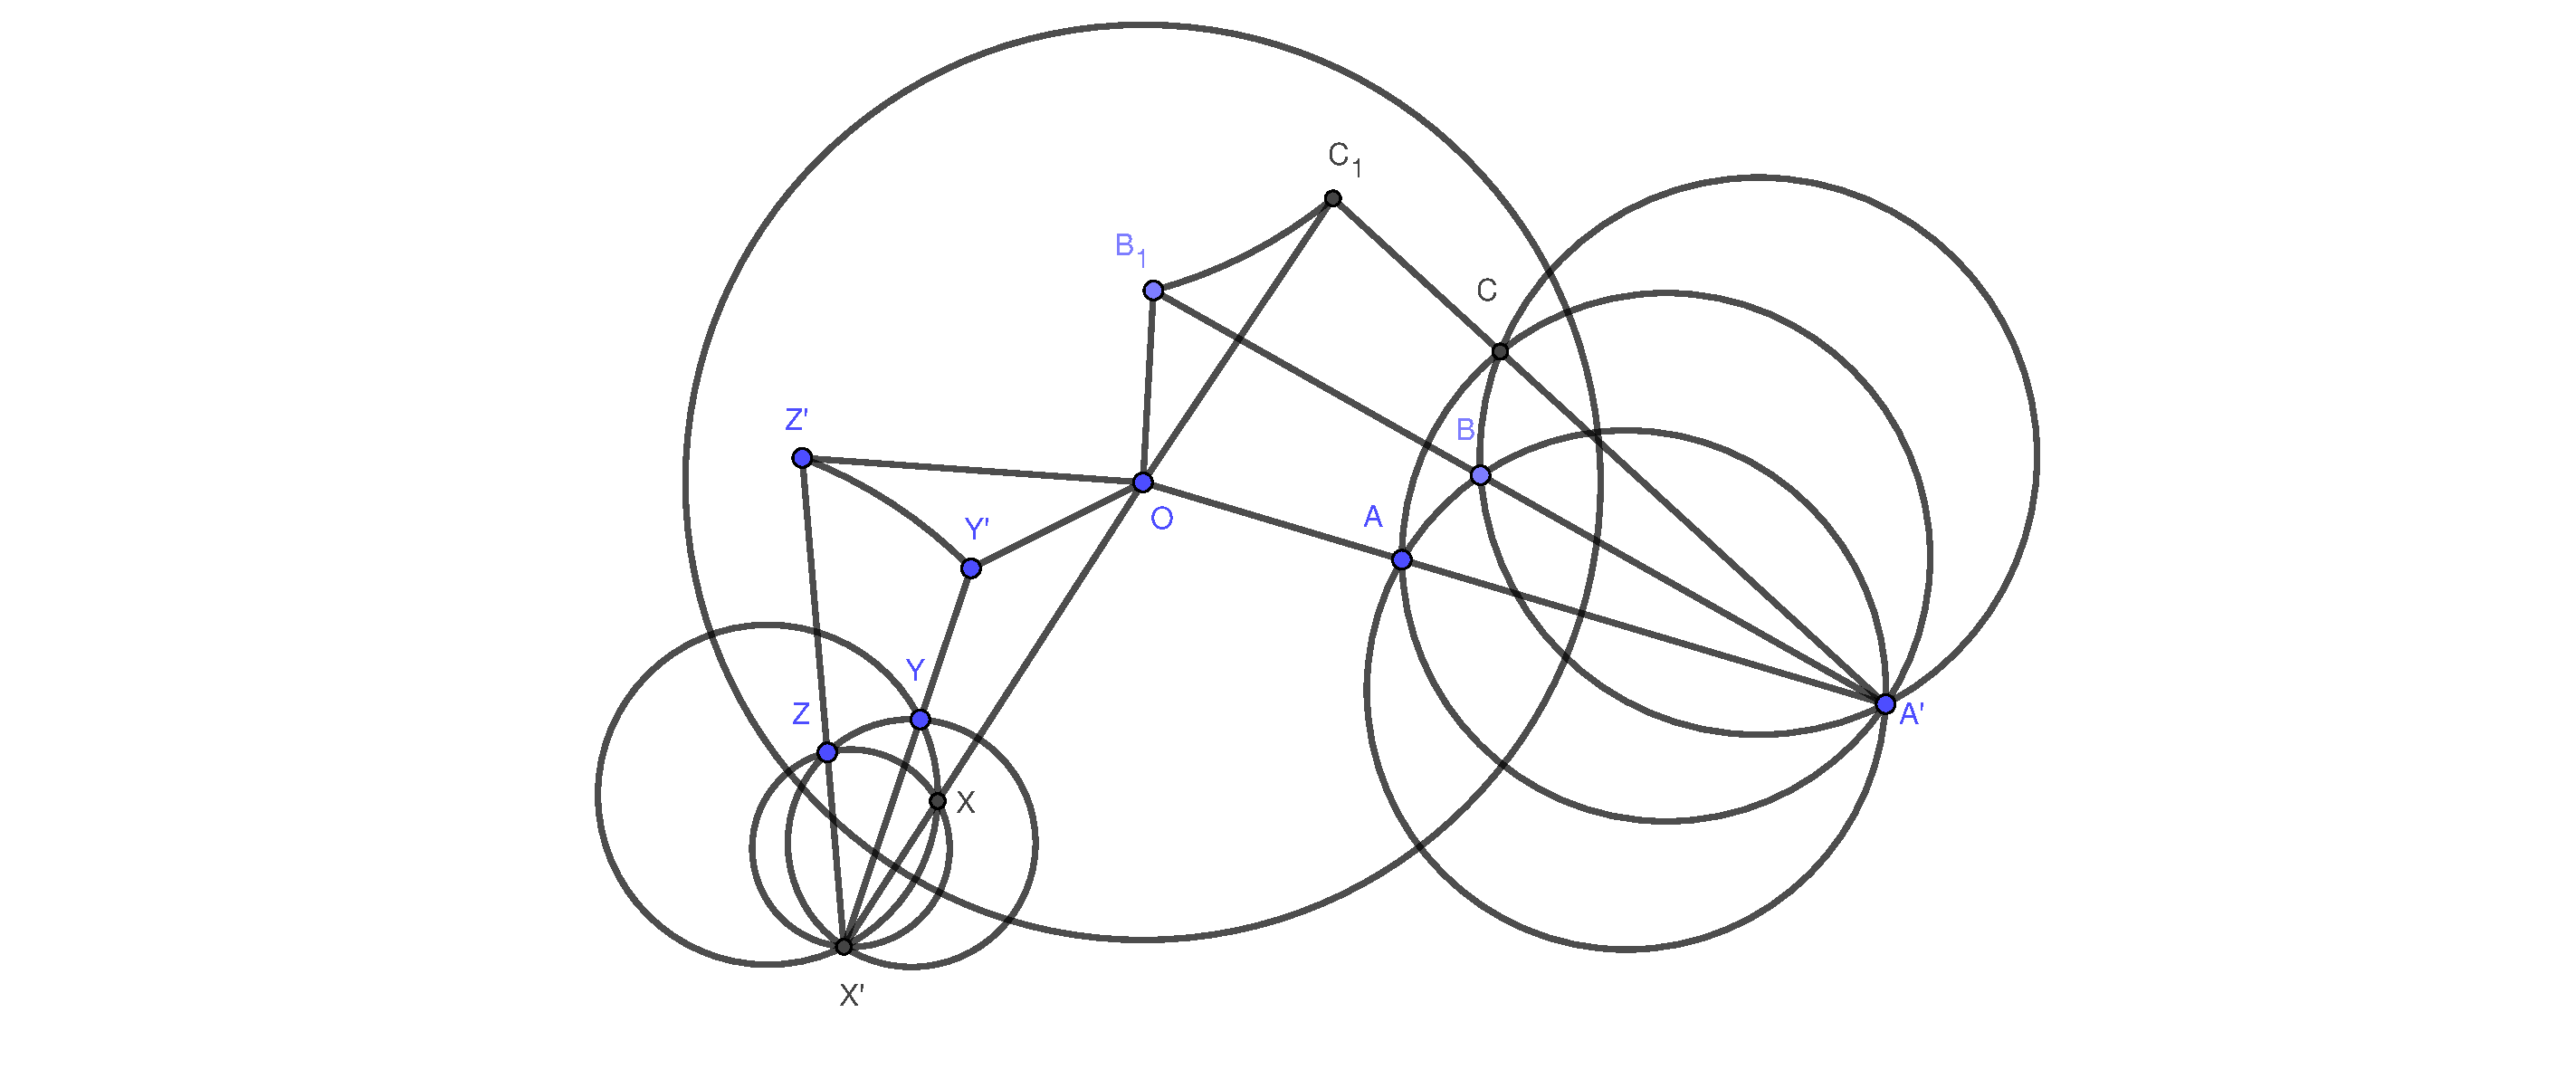
\includegraphics[width=\textwidth]{TH_cgc.pdf}
\end{figure}


\textit{Chứng minh.} Đầu tiên ta đưa bài toán về trường hợp đặc biệt A và X trùng O.
Theo chứng minh định lý xây dựng phép P-đối xứng, có một phép nghịch đảo biến A thành O nếu A khác O. Phép ấy sẽ biến $\Delta ABC$ thành $\Delta OB’C’$, và do tính bảo toàn góc và độ dài cạnh kiểu Poincar\'e của phép này, hai tam giác này bằng nhau. Để ý quan hệ bằng nhau của tam giác sẽ có tính bắc cầu từ việc quan hệ bằng nhau của góc và cạnh là bắc cầu. Một cách tương tự ta đẩy $\Delta XYZ$ về $ \Delta OY’Z’$.

Bổ đề sau đây sẽ chuyển sự bằng nhau của các đoạn Poincar\'e thành đoạn Euclid:

\textbf{Bổ đề 9.} \textit{Ta có: $OB =  r(e^d -1)/(e^d+1)$, ở đây r là bán kính của gamma, d = d(OB).}

\textit{Chứng minh}. Gọi hai đầu của đường Poincar\'e  OB là P và Q thỏa mãn 
Q - O - B - P, thì d = ln(OB, PQ).

Cho hai giá trị qua hàm mũ cơ số e:
\begin{eqnarray*}
e^d& = &(OB, PQ) = OP/OQ \cdot BQ/BP \textrm{(tất cả độ dài đại số)} \\
&= &
BQ/BP \textrm{(độ dài thường)}\\
& = &(r + OB)/(r-OB).
\end{eqnarray*} 
Từ đó ta thu được kết quả trên.
Ta chú ý vào hệ quả của nó: 
$$d(OX) = d(OY) 
\Longleftrightarrow OX = OY,$$ theo nghĩa Euclid.

Từ các kết quả trên, ta có: $OB’ = OY’, OC’ = OZ’, B’OC’ = Y’OZ’.$

Lúc này sẽ tồn tại một phép quay tâm O, hợp với một phép đối xứng qua một đường thẳng nào đó qua O nếu cần thiết (các phép biến hình của hình học Euclid) biến B’ thành Y’, C’ thành Z’, và bởi các phép này bảo toàn góc và độ dài cạnh, đường Poincar\'e qua B’C’ sẽ biến thành đường Poincar\'e qua Y’Z’, cho ta hai tam giác OB’C’ và OY’Z’ bằng nhau, hoàn tất chứng minh.

Ý tưởng này thật ra chính là đến từ lập luận ``dịch chuyển” của Euclid trong Định lý 4! Thế mới thấy ta có thể học hỏi được kể cả từ những chứng minh chưa chính xác!
 
Thật ra kết quả ta vừa chứng minh còn chi tiết hơn phát biểu ban đầu. Cụ thể là:

\textit{Hai tam giác bằng nhau kiểu Poincar\'e khi và chỉ khi có hữu hạn phép P-đối xứng nào đó để biến tam giác này thành tam giác kia.}


Điểm cuối cùng là Tiên đề về tính liên tục. May cho chúng ta là có một kết quả tốt trong mô hình Poincar\'e như sau:

\textbf{Định lý 10.}  \textit{Một đường tròn kiểu Poincar\'e chính là một đường tròn kiểu Euclid trong gamma, và ngược lại. Tuy nhiên tâm của đường tròn kiểu Poincar\'e chỉ trùng với tâm đường tròn kiểu Euclid khi nó là O.}

\textit{Chứng minh}. Nhận định sau được chứng minh nhờ vào hệ quả từ bổ đề trong chứng minh trường hợp cgc kiểu Poincar\'e phía trên. 
Xét trường hợp đường tròn Poincar\'e $\delta$ có tâm P là O’ khác O, sẽ tồn tại phép P-đối xứng f biến O’ thành O. Bởi phép P-đối xứng bảo toàn độ dài kiểu Poincar\'e, f(delta) sẽ là một đường tròn P có tâm là O, như vừa chỉ phía trên, đây chính là một đường tròn kiểu Euclid tâm O. Tác động lần nữa thì 
$f(f(\delta)) = \delta$ chính là một đường tròn Euclid, tuy nhiên có tâm khác O’.

Đảo lại với một đường tròn Euclid $\delta$ nào đó, gọi A, B là hai giao điểm của OO’ với $\delta$, và M là trung điểm của AB kiểu Poincar\'e. Khi ấy phép P-đối xứng biến M thành O có vai trò tương tự như f ở trường hợp trên. Thậm chí ta chứng minh được M chính là tâm Poincar\'e của delta.

\textbf{Hệ quả 11.}   \textit{Nguyên lý liên tục đường tròn - đường tròn đúng trong mô hình Poincar\'e.}

Tóm lại, qua những phát triển không ngắn gọn lắm vừa rồi, chúng ta đã dịch được các tiên đề của hình hyperbolic thành định lý của hình Euclid trong mô hình Poincar\'e. Điều đó là đủ để khẳng định: nếu hình học phẳng của Euclid không chứa mâu thuẫn, thì hình học hyperbolic cho mặt phẳng cũng vậy.


\begin{thebibliography}{99}
\bibitem{3}E.T.  Bell, \textit{Men of Mathematics The Lives and Achievements of the Great Mathematicians from Zeno to Poincaré}.   
\bibitem{4} David M. Burton. \textit{The History of Mathematics An Introduction}. 
\bibitem{2} M. J. Greenberg, \textit{Euclidean and Non-Euclidean Geometries - Development and History}. 
\bibitem{1} Wikipedia tiếng Anh.
\bibitem{5} https://www.youtube.com/playlist?list=PLjLK2cYtt-VBSBtvfhxx-DW3Zw3nOQHVZ  
\bibitem{6} https://rosetta.vn/lequanganh/wp-content/uploads/sites/7/2018/07/Riemann.pdf 
\bibitem{7} https://www.cut-the-knot.org/triangle/pythpar/Drama.shtml
\end{thebibliography} 
	